% !Mode:: "TeX:UTF-8"
% !TEX encoding = UTF-8 Unicode

%----------------------------------------------------------------------------------------
% 机器翻译:统计建模与深度学习方法
% Machine Translation: Statistical Modeling and Deep Learning Methods
%
% Copyright 2020
% 肖桐(xiaotong@mail.neu.edu.cn) 朱靖波 (zhujingbo@mail.neu.edu.cn)
%----------------------------------------------------------------------------------------

%----------------------------------------------------------------------------------------
%    CONFIGURATIONS
%----------------------------------------------------------------------------------------

\renewcommand\figurename{图}%将figure改为图
\renewcommand\tablename{表}%将figure改为图
%\renewcommand\arraystretch{1.5}%将表格高度调整为1.5倍
\chapterimage{../Figures/fig-NEU-3.jpg} % Chapter heading image

%----------------------------------------------------------------------------------------
%	CHAPTER 2
%----------------------------------------------------------------------------------------

\chapter{词法、语法及统计建模基础}

\parinterval 机器翻译并非是一个孤立的系统,它依赖于很多模块,并且需要很多学科知识的融合。现在的机器翻译系统大多使用统计模型对翻译问题进行建模,同时也会用到一些自然语言处理工具来对不同语言的文字进行分析。因此,在正式开始机器翻译内容的介绍之前,本章将会对相关的基础知识进行概述,包括:概率论与统计建模基础、语言分析、语言建模等。

\parinterval 概率论与统计建模是机器翻译方法的基础。这里会对机器翻译所涉及的基本数学概念进行简要描述,确保后续使用到的数学工具是完备的。本章会重点关注如何利用统计建模的方式对自然语言处理问题进行描述,这种手段在统计机器翻译和神经机器翻译中会被使用。

\parinterval 语言分析部分将以汉语为例介绍词法和句法分析的基本概念。它们都是自然语言处理中的经典问题,而且在机器翻译中也会经常被使用。同样,本章会介绍这两个任务的定义和求解问题的思路。

\parinterval 语言建模是机器翻译中最常用的一种技术,它主要用于句子的生成和流畅度评价。本章会以传统统计语言模型为例,对语言建模的相关概念进行介绍。但是,这里并不深入探讨语言模型技术,在后面的章节中还会单独对神经网络语言模型等前沿技术进行讨论。

%----------------------------------------------------------------------------------------
%    NEW SECTION
%----------------------------------------------------------------------------------------

\section{问题概述 }

\parinterval 很多时候机器翻译系统被看作是孤立的``黑盒''系统(图 \ref {fig:2-1} (a))。将一段文本作为输入送入机器翻译系统之后,系统输出翻译好的译文。但是真实的机器翻译系统非常复杂,因为系统看到的输入和输出实际上只是一些符号串,这些符号并没有任何意义,因此需要进一步对这些符号串进行处理才能更好的使用它们。比如,需要定义翻译中最基本的单元是什么?符号串是否具有结构信息?如何用数学工具刻画这些基本单元和结构?

%----------------------------------------------
\begin{figure}[htp]
    \centering
 	\subfigure[机器翻译系统被看作一个黑盒] {\definecolor{ublue}{rgb}{0.152,0.250,0.545}
\definecolor{ugreen}{rgb}{0,0.5,0}

%%% outline
%-------------------------------------------------------------------------

\vspace{0.3em}
\begin{tikzpicture}

\begin{scope}
\node [] (input) at (0,0) {{\scriptsize 猫喜欢吃鱼}};

\node [] (output) at ([xshift=3.35in]input.east) {{\scriptsize Cats like eating fish}};

\draw[->,thick] ([xshift=-1pt]input.east) -- ([xshift=8pt]input.east);
\draw[->,thick] ([xshift=-10pt]output.west) -- ([xshift=-0pt]output.west);

%{
%\draw[->,thick] ([xshift=-12pt]mtengine.west) -- ([xshift=-2pt]mtengine.west);
%\draw[->,thick] ([xshift=2pt]mtengine.east) -- ([xshift=12pt]mtengine.east);
%}

{
\node[minimum height=4em,minimum width=4.5em,fill=white] (inputmarking) at (0.88in,-0.39in) {};
\node[minimum height=4em,minimum width=5.2em,fill=white] (outputmarking) at (2.57in,-0.39in) {};
}

\node [anchor=south] (inputlabel) at ([yshift=-0.5em]input.north) {{\scriptsize \color{red}{\textbf{输入}}}};
\node [anchor=south] (outputlabel) at ([yshift=-0.5em]output.north) {{\scriptsize \color{red}{\textbf{输出}}}};

{
\node [anchor=west] (mtinputlabel) at ([xshift=0.32in]inputlabel.east) {{\scriptsize \color{red}{\textbf{}}}};
\node [anchor=west] (mtoutputlabel) at ([xshift=0.88in]mtinputlabel.east) {{\scriptsize \color{red}{\textbf{}}}};
\node[rectangle,draw=ublue, inner sep=0mm] [fit = (mtinputlabel) (mtoutputlabel) (inputmarking) (outputmarking)] {};
}

{
\node[rectangle,fill=ublue,inner sep=0mm] [fit = (mtinputlabel) (mtoutputlabel) (inputmarking) (outputmarking)] {{\color{white} \textbf{\Large{MT 系统}}}};
}


%\begin{scope}[scale=0.9,xshift=1.2in,yshift=-1.2in,level distance=20pt,sibling distance=0pt]
%
%\end{scope}

\end{scope}

\end{tikzpicture}




  }
 	\subfigure[机器翻译系统 = 前/后处理 + 翻译引擎] {\definecolor{ublue}{rgb}{0.152,0.250,0.545}
\definecolor{ugreen}{rgb}{0,0.5,0}

%%% outline
%-------------------------------------------------------------------------

\vspace{0.3em}
\begin{tikzpicture}

\begin{scope}
\node [] (input) at (0,0) {{\scriptsize 猫喜欢吃鱼}};

{
\begin{scope}[scale=0.8,xshift=0.9in,yshift=-0.87in,level distance=20pt,sibling distance=-1pt,grow'=up]
{\scriptsize
\Tree[.\node(sn0){IP};
          [.\node(sn1){NP};
               [.\node(sn2){NN}; \node(sw1){猫}; ]
          ]
          [.\node(sn3){VP};
               [.\node(sn4){VV}; \node(sw2){喜欢}; ]
               [.\node(sn5){VP}; \edge[roof]; \node(sw3){吃 \ 鱼}; ]
          ]
     ]
}
\end{scope}

\node [anchor=west,draw,thick,inner sep=3pt,ublue] (mtengine) at ([xshift=1.05in]input.east) {{\scriptsize MT系统}};

\begin{scope}[scale=0.8,xshift=3.0in,yshift=-0.87in,level distance=20pt,sibling distance=-3pt,grow'=up]
{\scriptsize
\Tree[.\node(tn0){S};
          [.\node(tn1){NP};
               [.\node(tn2){NNS}; \node(tw1){cats}; ]
          ]
          [.\node(tn3){VP};
               [.\node(tn4){VB}; \node(tw2){like}; ]
               [.\node(tn5){VP}; \edge[roof]; \node(tw3){eating fish}; ]
          ]
     ]
}

\end{scope}
}

\node [] (output) at ([xshift=3.35in]input.east) {{\scriptsize Cats like eating fish}};

\draw[->,thick] ([xshift=-1pt]input.east) -- ([xshift=8pt]input.east);
\draw[->,thick] ([xshift=-10pt]output.west) -- ([xshift=-0pt]output.west);

{
\draw[->,thick] ([xshift=-12pt]mtengine.west) -- ([xshift=-2pt]mtengine.west);
\draw[->,thick] ([xshift=2pt]mtengine.east) -- ([xshift=12pt]mtengine.east);
}

{
\node[minimum height=4em,minimum width=4.5em] (inputmarking) at (0.85in,-0.39in) {};
\node[minimum height=4em,minimum width=5.2em] (outputmarking) at (2.55in,-0.39in) {};
}

\node [anchor=south] (inputlabel) at ([yshift=-0.5em]input.north) {{\scriptsize \color{red}{\textbf{输入}}}};
\node [anchor=south] (outputlabel) at ([yshift=-0.5em]output.north) {{\scriptsize \color{red}{\textbf{输出}}}};

{
\node [anchor=west] (mtinputlabel) at ([xshift=0.29in]inputlabel.east) {{\scriptsize \color{red}{\textbf{实际的输入}}}};
\node [anchor=west] (mtoutputlabel) at ([xshift=1.0in]mtinputlabel.east) {{\scriptsize \color{red}{\textbf{实际的输出}}}};
\node[rectangle,draw=ublue, inner sep=0mm] [fit = (mtinputlabel) (mtoutputlabel) (inputmarking) (outputmarking)] {};
}

\end{scope}

\end{tikzpicture}




}
	\caption{机器翻译系统的结构}
    \label{fig:2-1}
\end{figure}
%-------------------------------------------

%----------------------------------------------
\begin{figure}[htp]
\centering
\input{./Chapter2/Figures/figure-analysis-of-sentence-participle&syntactic}
\caption{中文句子``猫喜欢吃鱼''的分析结果(分词和句法分析)}
\label{fig:2-2}
\end{figure}
%-------------------------------------------

\parinterval 图\ref{fig:2-1} (b)展示了一个机器翻译系统的输入和输出形式。可以看到,输入的中文词串``猫喜欢吃鱼''被加工成一个新的结构(图\ref {fig:2-2})。直觉上,这个结构有些奇怪,因为上面多了很多新的符号,而且还有一些线将不同符号进行连接。实际上这就是语言分析中对句子常用的结构表示 —— 短语结构树。从原始的词串转化为图\ref {fig:2-2} 的样子,有两个步骤:

\begin{itemize}
\vspace{0.5em}
\item {\small\bfnew{分词}}\index{分词}(Segmentation)\index{Segmentation}:这个过程会把词串进行切分,切割成最小的单元。因为只有知道了什么是待处理字符串的最小单元,机器翻译系统才能对其进行表示、分析和生成。
\vspace{0.5em}
\item {\small\bfnew{句法分析}}\index{句法分析}(Parsing)\index{Parsing}:这个过程会对分词的结果进行进一步分析,得到句子的句法结构。这种结构是对句子的进一步抽象,比如,NP+VP就可以表示由名词短语(NP)和动词短语(VP)构成的主谓结构。利用这些信息,机器翻译可以更加准确地对语言的结构进行分析和生成。
\vspace{0.5em}
\end{itemize}

\parinterval 类似地,机器翻译输出的结果也可以包含同样的信息。甚至系统输出英文译文之后,还有一个额外的步骤来把部分英文单词的大小写恢复出来,比如,上例中句首单词Cats的首字母要大写。

\parinterval 一般来说,在送入机器翻译系统前需要对文字序列进行处理和加工,这个过程被称为{\small\sffamily\bfseries{预处理}}\index{预处理}(Pre-processing)\index{Pre-processing}。同理,在机器翻译模型输出译文后进行的处理被称作{\small\sffamily\bfseries{后处理}}\index{后处理}(Post-processing)\index{Post-processing}。这两个过程对机器翻译性能影响很大,比如,在神经机器翻译里,不同的分词策略可能会造成翻译性能的天差地别。

\parinterval 值得注意的是,有些观点认为,不论是分词还是句法分析,对于机器翻译来说并不要求符合人的认知和语言学约束。换句话说,机器翻译所使用的``单词''和``结构''本身并不是为了符合人类的解释,它们更直接目的是为了进行翻译。从系统开发的角度,有时候即使是一些与人类的语言习惯有差别的处理,仍然会带来性能的提升,比如在神经机器翻译中,在传统分词的基础上进一步使用双字节编码(Byte Pair Encoding,BPE)子词切分会使得机器翻译性能大幅提高。当然,自然语言处理中语言学信息的使用一直是学界关注的焦点。甚至关于语言学结构对机器翻译是否有作用这个问题也有争论。但是不能否认的是,无论是语言学的知识,还是计算机自己学习到的知识,对机器翻译都是有价值的。在后续章节会看到,这两种类型的知识对机器翻译帮助很大 \footnote[1]{笔者并不认同语言学结构对机器翻译的帮助有限,相反机器翻译需要更多的人类先验知识的指导。当然,这个问题不是这里讨论的重点。} 。

\parinterval 剩下的问题是如何进行句子的切分和结构的分析。思路有很多,一种常用的方法是对问题进行概率化,用统计模型来描述问题并求解之。比如,一个句子切分的好坏,并不是非零即一的判断,而是要估计出这种切分的可能性大小,最终选择可能性最大的结果进行输出。这也是一种典型的用统计建模的方式来描述自然语言处理问题的方法。

\parinterval 本章将会对上述问题及求解问题的方法进行介绍。首先,会用一个例子给出统计建模的基本思路,之后会应用这种方法进行中文分词、语言建模和句法分析。
\vspace{-1em}

%----------------------------------------------------------------------------------------
%    NEW SECTION
%----------------------------------------------------------------------------------------

\sectionnewpage
\section{概率论基础}
\parinterval 为了便于后续内容的介绍,首先对本书中使用的概率和统计学概念进行说明。

%----------------------------------------------------------------------------------------
%    NEW SUB-SECTION
%----------------------------------------------------------------------------------------

\subsection{随机变量和概率}
\parinterval 在自然界中,很多{\small\bfnew{事件}}\index{事件}(Event)\index{Event}是否会发生是不确定的。例如,明天会下雨、掷一枚硬币是正面朝上、扔一个骰子的点数是5$\cdots\cdots$这类事件可能会发生也可能不会发生。通过大量的重复试验,能发现其具有某种规律性的事件叫做{\small\sffamily\bfseries{随机事件}}\index{随机事件}。

\parinterval {\small\sffamily\bfseries{随机变量}}\index{随机变量}(Random Variable)\index{Random Variable}是对随机事件发生可能状态的描述,是随机事件的数量表征。设$\Omega = \{ \omega \}$为一个随机试验的样本空间,$X=X(\omega)$就是定义在样本空间$\Omega$上的单值实数函数,即$X=X(\omega)$为随机变量,记为$X$。随机变量是一种能随机选取数值的变量,常用大写的英文字母或希腊字母表示,其取值通常用小写字母来表示。例如,用$A$ 表示一个随机变量,用$a$表示变量$A$的一个取值。根据随机变量可以选取的值的某些性质,可以将其划分为离散变量和连续变量。

\parinterval 离散变量是指在其取值区间内可以被一一列举,总数有限并且可计算的数值变量。例如,用随机变量$X$代表某次投骰子出现的点数,点数只可能取1$\sim$6这6个整数,$X$就是一个离散变量。

\parinterval 连续变量是在其取值区间内连续取值,无法被一一列举,具有无限个取值的变量。例如,图书馆的开馆时间是8:30-22:00,用$X$代表某人进入图书馆的时间,时间的取值范围是[8:30,22:00]这个时间区间,$X$就是一个连续变量。

\parinterval {\small\bfnew{概率}}\index{概率}(Probability)\index{Probability}是度量随机事件呈现其每个可能状态的可能性的数值,本质上它是一个测度函数\cite{mao-prob-book-2011}\cite{kolmogorov2018foundations}。概率的大小表征了随机事件在一次试验中发生的可能性大小。用$\textrm{P}(\cdot )$表示一个随机事件的可能性,即事件发生的概率。比如$\textrm{P}(\textrm{太阳从东方升起})$表示``太阳从东方升起的可能性'',同理,$\textrm{P}(A=B)$ 表示的就是``$A=B$'' 这件事的可能性。

\parinterval 在实际问题中,往往需要得到随机变量的概率值。但是,真实的概率值可能是无法准确知道的,这时就需要对概率进行{\small\sffamily\bfseries{估计}}\index{估计},得到的结果是概率的{\small\sffamily\bfseries{估计值}}\index{估计值}(Estimate)\index{Estimate}。在概率论中,一个很简单的方法是利用相对频度作为概率的估计值。如果$\{x_1,x_2,\dots,x_n \}$是一个试验的样本空间,在相同情况下重复试验$N$次,观察到样本$x_i (1\leq{i}\leq{n})$的次数为$n (x_i )$,那么$x_i$在这$N$次试验中的相对频率是$\frac{n(x_i )}{N}$。当$N$越来越大时,相对概率也就越来越接近真实概率$\textrm{P}(x_i)$,即$\lim_{N \to \infty}\frac{n(x_i )}{N}=\textrm{P}(x_i)$。 实际上,很多概率模型都等同于相对频度估计,比如,对于一个服从多项式分布的变量的极大似然估计就可以用相对频度估计实现。

%--------------------------------------------------------------------
\begin{table}[htp]
\centering
\caption{离散变量$A$的概率分布}
\begin{tabular}{c|c c c c c c}
\rule{0pt}{15pt}     $A$ & $a_1=1$ & $a_2=2$ & $a_3=3$ & $a_4=4$ & $a_5=5$ & $a_6=6$\\
               \hline
\rule{0pt}{15pt}     $\textrm{P}_i$ & $\textrm{P}_1=\frac{4}{25}$  &  $\textrm{P}_2=\frac{3}{25}$ &  $\textrm{P}_3=\frac{4}{25}$ & $\textrm{P}_4=\frac{6}{25}$ & $\textrm{P}_5=\frac{3}{25}$ & $\textrm{P}_6=\frac{1}{25}$  \\
             \end{tabular}
             \label{tab:2-1}
\end{table}
%--------------------------------------------------------------------

\parinterval 概率函数是用函数形式给出离散变量每个取值发生的概率,其实就是将变量的概率分布转化为数学表达形式。如果把$A$看做一个离散变量,$a$看做变量$A$的一个取值,那么$\textrm{P}(A)$被称作变量$A$的概率函数,$\textrm{P}(A=a)$被称作$A = a$的概率值,简记为$\textrm{P}(a)$。例如,在相同条件下掷一个骰子50次,用$A$表示投骰子出现的点数这个离散变量,$a_i$表示点数的取值,$\textrm{P}_i$表示$A=a_i$的概率值。表\ref{tab:2-1}为$A$的概率分布,给出了$A$的所有取值及其概率。

\parinterval 除此之外,概率函数$\textrm{P}(\cdot)$还具有非负性、归一性等特点。非负性是指,所有的概率函数$\textrm{P}(\cdot)$都必须是大于等于0的数值,概率函数中不可能出现负数,即$\forall{x},\textrm{P}{(x)}\geq{0}$。归一性,又称规范性,简单的说就是所有可能发生的事件的概率总和为1,即$\sum_{x}\textrm{P}{(x)}={1}$。

%----------------------------------------------
\begin{figure}[htp]
\centering
 
%%% outline
%-------------------------------------------------------------------------
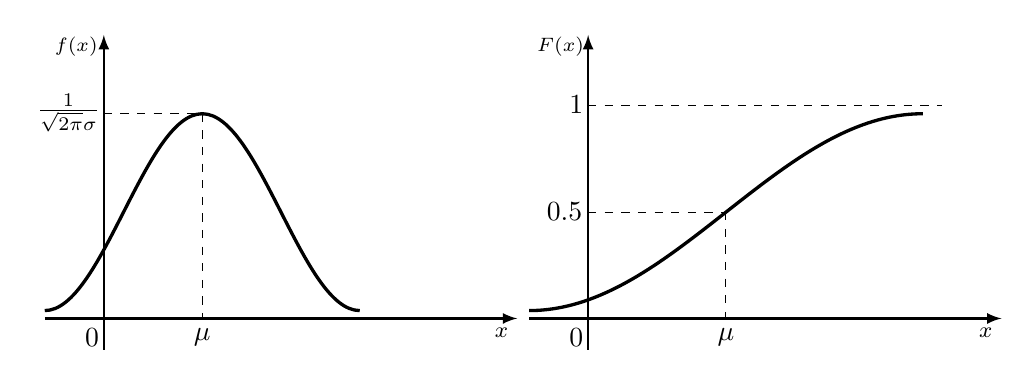
\begin{tikzpicture}


\begin{scope}[scale=0.5]

\draw [-,very thick] (-2,-1) cos(0,1.5) sin (2,4) cos(4,1.5) sin(6,-1) ;
\draw [-latex,thick] (-2.0,-1.2) -- (10,-1.2);%横轴
\draw [-latex,thick] (-0.5,-2.0) -- (-0.5,6);%纵轴
\draw [-,dashed] (2,4) -- (2,-1.2);  %%图中纵轴虚线
\draw [-,dashed] (-0.5,4) -- (2,4);  %%图中横轴虚线
\node [anchor=north] at (-0.8,-1.2) {0};
\node [anchor=north] at (2,-1.2) {$\mu$};
\node [anchor=north] at (-1.4,4.75) {$\frac{1}{\sqrt{2\pi}\sigma}$};
\node [anchor=north] at (-1.2,6.2) {\scriptsize{$f(x)$}};
\node [anchor=north] at (9.6,-1.2) {\footnotesize{$x$}};


\end{scope}

\begin{scope}[scale=0.5,xshift=35.0em]

\draw [-,very thick] (-2,-1) cos(3,1.5) sin(8,4) ;
\draw [-latex,thick] (-2.0,-1.2) -- (10,-1.2);%横轴
\draw [-latex,thick] (-0.5,-2.0) -- (-0.5,6.0);%纵轴
\draw [-,dashed] (3,1.5) -- (3,-1.2);  %%图中纵轴虚线
\draw [-,dashed] (-0.5,1.5) -- (3,1.5);  %%图中横轴虚线
\draw [-,dashed] (-0.5,4.2) -- (8.5,4.2);  %%图中横轴虚线
\node [anchor=north] at (-0.8,-1.2) {0};
\node [anchor=north] at (3,-1.2) {$\mu$};
\node [anchor=north] at (-1.1,2.0) {0.5};
\node [anchor=north] at (-0.8,4.7) {1};
\node [anchor=north] at (-1.2,6.2) {\scriptsize{$F(x)$}};
\node [anchor=north] at (9.6,-1.2) {\footnotesize{$x$}};

\end{scope}


\end{tikzpicture}
%---------------------------------------------------------------------




\caption{一个概率密度函数(左)与其对应的分布函数(右)}
\label{fig:2-3}
\end{figure}
%-------------------------------------------

\parinterval 对于离散变量$A$,$\textrm{P}(A=a)$是个确定的值,可以表示事件$A=a$的可能性大小;而对于连续变量,求在某个定点处的概率是无意义的,只能求其落在某个取值区间内的概率。因此,用{\small\sffamily\bfseries{概率分布函数}}\index{概率分布函数}$F(x)$和{\small\sffamily\bfseries{概率密度函数}}\index{概率密度函数}$f(x)$来统一描述随机变量取值的分布情况(如图\ref{fig:2-3})。概率分布函数$F(x)$表示取值小于等于某个值的概率,是概率的累加(或积分)形式。假设$A$是一个随机变量,$a$是任意实数,将函数$F(a)=\textrm{P}\{A\leq a\}$,$-\infty<a<\infty $定义为$A$的分布函数。通过分布函数,可以清晰地表示任何随机变量的概率。

\parinterval 概率密度函数反映了变量在某个区间内的概率变化快慢,概率密度函数的值是概率的变化率,该连续变量的概率也就是对概率密度函数求积分得到的结果。设$f(x) \geq 0$是连续变量$X$的概率密度函数,$X$的分布函数就可以用如下公式定义:
\begin{eqnarray}
F(x)=\int_{-\infty}^x f(x)dx
\label{eq:2-1}
\end{eqnarray}

%----------------------------------------------------------------------------------------
%    NEW SUB-SECTION
%----------------------------------------------------------------------------------------

\subsection{联合概率、条件概率和边缘概率}
\parinterval {\small\sffamily\bfseries{联合概率}}\index{联合概率}(Joint Probability)\index{Joint Probability}是指多个事件共同发生,每个随机变量满足各自条件的概率,表示为$\textrm{P}(AB)$或$\textrm{P}(A\cap{B})$。{\small\sffamily\bfseries{条件概率}}\index{条件概率}(Conditional Probability)\index{Conditional Probability}是指$A$、$B$为任意的两个事件,在事件$A$已出现的前提下,事件$B$出现的概率,使用$\textrm{P}(B \mid A)$表示。

\parinterval 贝叶斯法则(见\ref{sec:2.2.3}小节)是条件概率计算时的重要依据,条件概率可以表示为
\begin{eqnarray}
\textrm{P}{(B|A)} & = & \frac{\textrm{P}(A\cap{B})}{\textrm{P}(A)}  \nonumber \\
                           & = & \frac{\textrm{P}(A)\textrm{P}(B|A)}{\textrm{P}(A)}  \nonumber \\
                           & = & \frac{\textrm{P}(B)\textrm{P}(A|B)}{\textrm{P}(A)}
\label{eq:2-2}
\end{eqnarray}

\parinterval {\small\sffamily\bfseries{边缘概率}}\index{边缘概率}(marginal probability)\index{marginal probability}是和联合概率对应的,它指的是$\textrm{P}(X=a)$或$\textrm{P}(Y=b)$,即仅与单个随机变量有关的概率。对于离散随机变量$X$和$Y$,如果知道$\textrm{P}(X,Y)$,则边缘概率$\textrm{P}(X)$可以通过求和的方式得到。对于$\forall x \in X $,有
\begin{eqnarray}
\textrm{P}(X=x)=\sum_{y}  \textrm{P}(X=x,Y=y)
\label{eq:2-3}
\end{eqnarray}

\parinterval 对于连续变量,边缘概率$\textrm{P}(X)$需要通过积分得到,如下式所示
\begin{eqnarray}
\textrm{P}(X=x)=\int \textrm{P}(x,y)dy
\label{eq:2-4}
\end{eqnarray}

\parinterval 为了更好地区分条件概率、边缘概率和联合概率,这里用一个图形面积的计算来举例说明。如图\ref{fig:2-4}所示,矩形$A$代表事件$X$发生所对应的所有可能状态,矩形$B$代表事件$Y$发生所对应的所有可能状态,矩形$C$代表$A$和$B$的交集,则

\begin{itemize}
\vspace{0.5em}
\item 边缘概率:矩形$A$或者矩形$B$的面积;
\vspace{0.5em}
\item 联合概率:矩形$C$的面积;
\vspace{0.5em}
\item 条件概率:联合概率/对应的边缘概率,如:$\textrm{P}(A \mid B)$=矩形$C$的面积/矩形B的面积。
\vspace{0.5em}
\end{itemize}

%----------------------------------------------
\begin{figure}[htp]
\centering
\input{./Chapter2/Figures/figure-schematic-edge-probability&joint-probability}
\caption{$A$、$B$、$C$事件所对应概率的图形化表示}
\label{fig:2-4}
\end{figure}
%-------------------------------------------

%----------------------------------------------------------------------------------------
%    NEW SUB-SECTION
%----------------------------------------------------------------------------------------

\subsection{链式法则}

\parinterval 条件概率公式$\textrm{P}(A \mid B)=\textrm{P}(AB)/\textrm{P}(B)$反映了事件$B$发生的条件下事件$A$发生的概率。如果将其推广到三个事件$A$、$B$、$C$,为了计算$\textrm{P}(A,B,C)$,我们可以运用两次$\textrm{P}(A \mid B)=\textrm{P}(AB)/\textrm{P}(B)$,计算过程如下:
\begin{eqnarray}
\textrm{P}(A,B,C) & = & \textrm{P}(A \mid B ,C)\textrm{P}(B,C) \nonumber \\
                           & = & \textrm{P}(A \mid B,C)\textrm{P}(B \mid C)\textrm{P}(C)
\label{eq:2-5}
\end{eqnarray}

\parinterval 推广到$n$个事件,可以得到了链式法则的公式
\begin{eqnarray}
\textrm{P}(x_1,x_2,...,x_n)=\textrm{P}(x_1) \prod_{i=2}^n \textrm{P}(x_i \mid x_1,x_2,...,x_{i-1})
\label{eq:2-6}
\end{eqnarray}

\parinterval 下面的例子有助于更好的理解链式法则,如图\ref{fig:2-5}所示,$A$、$B$、$C$、$D$、\\ $E$分别代表五个事件,其中,$A$只和$B$有关,$C$只和$B$、$D$有关,$E$只和$C$有关,$B$和$D$不依赖其他任何事件。则$\textrm{P}(A,B,C,D,E)$的表达式如下式:

%----------------------------------------------
\begin{figure}[htp]
\centering
\input{./Chapter2/Figures/figure-schematic-chain-rule}
\setlength{\belowcaptionskip}{-1cm}
\caption{事件$A$、$B$、$C$、$D$、$E$之间的关系图}
\label{fig:2-5}
\end{figure}
%-------------------------------------------

\begin{eqnarray}
&   & \textrm{P}(A,B,C,D,E) \nonumber \\
&=&\textrm{P}(E \mid A,B,C,D) \cdot \textrm{P}(A,B,C,D) \nonumber \\
&=&\textrm{P}(E \mid A,B,C,D) \cdot \textrm{P}(D \mid A,B,C) \cdot \textrm{P}(A,B,C) \nonumber \\
&=&\textrm{P}(E \mid A,B,C,D) \cdot \textrm{P}(D \mid A,B,C) \cdot \textrm{P}(C \mid A,B) \cdot \textrm{P}(A,B) \nonumber \\
&=&\textrm{P}(E \mid A,B,C,D) \cdot \textrm{P}(D \mid A,B,C) \cdot \textrm{P}(C \mid A,B) \cdot \textrm{P}(B \mid A) \cdot \textrm{P}(A)
\label{eq:2-7}
\end{eqnarray}

\parinterval 根据图\ref {fig:2-5} 易知$E$只和$C$有关,所以$\textrm{P}(E \mid A,B,C,D)=\textrm{P}(E \mid C)$;$D$不依赖于其他事件,所以$\textrm{P}(D \mid A,B,C)=\textrm{P}(D)$;$C$只和$B$、$D$有关,所以$\textrm{P}(C \mid A,B)=\textrm{P}(C \mid B)$;$B$不依赖于其他事件,所以$\textrm{P}(B \mid  A)=\textrm{P}(B)$。最终化简可得:
\begin{eqnarray}
\textrm{P}(A,B,C,D,E)=\textrm{P}(E \mid C) \cdot \textrm{P}(D) \cdot \textrm{P}(C \mid B) \cdot \textrm{P}(B)\cdot \textrm{P}(A \mid B)
\label{eq:2-8}
\end{eqnarray}

%----------------------------------------------------------------------------------------
%    NEW SUB-SECTION
%----------------------------------------------------------------------------------------

\subsection{贝叶斯法则}\label{sec:2.2.3}

\parinterval 首先介绍一下全概率公式:{\small\bfnew{全概率公式}}\index{全概率公式}(Law of Total Probability)\index{Law of Total Probability}是概率论中重要的公式,它可以将一个复杂事件发生的概率分解成不同情况的小事件发生概率的和。这里先介绍一个概念——划分。集合$S$的一个划分事件为$\{B_1,...,B_n\}$是指它们满足$\bigcup_{i=1}^n B_i=S \textrm{且}B_iB_j=\varnothing , i,j=1,...,n,i\neq j$。此时事件$A$的全概率公式可以被描述为:

\begin{eqnarray}
\textrm{P}(A)=\sum_{k=1}^n \textrm{P}(A \mid B_k)\textrm{P}(B_k)
\label{eq:2-9}
\end{eqnarray}

\parinterval 举个例子,小张从家到公司有三条路分别为$a$,$b$,$c$,选择每条路的概率分别为0.5,0.3,0.2。令:

\begin{itemize}
\vspace{0.5em}
\item $S_a$:小张选择$a$路去上班
\vspace{0.5em}
\item $S_b$:小张选择$b$路去上班
\vspace{0.5em}
\item $S_c$:小张选择$c$路去上班
\vspace{0.5em}
\item $S$:小张去上班
\vspace{0.5em}
\end{itemize}

\parinterval 显然,$S_a$,$S_b$,$S_c$是$S$的划分。如果三条路不拥堵的概率分别为$\textrm{P}({S_{a}^{'}})$=0.2, $\textrm{P}({S_{b}^{'}})$=0.4,$\textrm{P}({S_{c}^{'}})$=0.7,那么事件$L$:小张上班没有遇到拥堵情况的概率就是:
\begin{eqnarray}
{\textrm{P}(L)} &=& {\textrm{P}( L| S_a )\textrm{P}(S_a )+\textrm{P}( L| S_b )\textrm{P}(S_b )+\textrm{P}( L| S_c )\textrm{P}(S_c )}\nonumber \\
& = &{\textrm{P}({S_{a}^{'}})\textrm{P}(S_a)+\textrm{P}({S_{b}^{'}})\textrm{P}(S_b)+\textrm{P}({S_{c}^{'}})\textrm{P}(S_c) }\nonumber \\
& = &{0.36}
\label{eq:2-10}
\end{eqnarray}

\parinterval {\small\sffamily\bfseries{贝叶斯法则}}\index{贝叶斯法则}(Bayes' rule)\index{Bayes' rule}是概率论中的一个经典公式,通常用于已知$\textrm{P}(A \mid B)$求$\textrm{P}(B \mid A)$。可以表述为:设$\{B_1,...,B_n\}$是$S$的一个划分,$A$为事件,则对于$i=1,...,n$,有如下公式
\begin{eqnarray}
\textrm{P}(B_i \mid A) & = & \frac {\textrm{P}(A  B_i)} { \textrm{P}(A) } \nonumber \\
                                   & = & \frac {\textrm{P}(A \mid B_i)\textrm{P}(B_i) } { \sum_{k=1}^n\textrm{P}(A \mid B_k)\textrm{P}(B_k) }
\label{eq:2-11}
\end{eqnarray}

\noindent 其中,等式右端的分母部分使用了全概率公式。由上式,也可以得到贝叶斯公式的另外两种写法:
\begin{eqnarray}
\textrm{P}(B \mid A) & = & \frac { \textrm{P}(A \mid B)\textrm{P}(B) }  {\textrm{P}(A)} \nonumber \\
                     & = & \frac { \textrm{P}(A \mid B)\textrm{P}(B) }  {\textrm{P}(A \mid B)\textrm{P}(B)+\textrm{P}(A \mid \bar{B}) \textrm{P}(\bar{B})}
\label{eq:2-12}
\end{eqnarray}

\parinterval 贝叶斯公式常用于根据已知的结果来推断使之发生的各因素的可能性。 \\ \\ 

%----------------------------------------------------------------------------------------
%    NEW SUB-SECTION
%----------------------------------------------------------------------------------------

\subsection{KL距离和熵}

%----------------------------------------------------------------------------------------
%    NEW SUBSUB-SECTION
%----------------------------------------------------------------------------------------

\subsubsection{信息熵}

\parinterval {\small\sffamily\bfseries{熵}}\index{熵}(Entropy)\index{Entropy}是热力学中的一个概念,同时也是对系统无序性的一种度量标准。在自然语言处理领域也会使用到信息熵这一概念,比如描述文字的信息量大小。一条信息的信息量可以被看作是这条信息的不确定性。如果需要确认一件非常不确定甚至于一无所知的事情,那么需要理解大量的相关信息才能进行确认;同样的,如果对某件事已经非常确定,那么就不需要太多的信息就可以把它搞清楚。如下就是两个例子,

\begin{example}
确定性和不确定性的事件

\qquad\qquad\quad``太阳从东方升起''

\qquad\qquad\quad``明天天气多云''
\label{eg:2-1}
\end{example}

\parinterval 在这两句话中,``太阳从东方升起''是一件确定性事件(在地球上),几乎不需要查阅更多信息就可以确认,因此这件事的信息熵相对较低;而``明天天气多云''这件事,需要关注天气预报,才能大概率确定这件事,它的不确定性很高,因而它的信息熵也就相对较高。因此,信息熵也是对事件不确定性的度量。进一步,定义{\small\bfnew{自信息}}\index{自信息}(Self-information)\index{Self-information}为一个事件$X$的自信息的表达式为:
\begin{eqnarray}
\textrm{I}(x)=-\log\textrm{P}(x)
\label{eq:2-13}
\end{eqnarray}

\noindent 其中,$\textrm{P}(x)$表示$x$发生的概率。自信息用来衡量单一事件发生时所包含的信息多少,当底数为e时,单位为nats,其中1nats是通过观察概率为$\frac{1}{e}$的事件而获得的信息量;当底数为2 时,单位为bits或shannons。$\textrm{I}(x)$和$\textrm{P}(x)$的函数关系如图\ref{fig:2-6} 所示。

%----------------------------------------------
\begin{figure}[htp]
\centering
\input{./Chapter2/Figures/figure-self-information-function}
\caption{自信息函数$\textrm{I}(x)$关于$\textrm{P}(x)$的曲线}
\label{fig:2-6}
\end{figure}
%-------------------------------------------

\parinterval 自信息处理的是变量单一取值的情况。若量化整个概率分布中的不确定性或信息量,可以用信息熵,记为$\textrm{H}(x)$。其公式如下:
\begin{eqnarray}
\textrm{H}(x) & = & \sum_{x \in \textrm{X}}[ \textrm{P}(x) \textrm{I}(x)] \nonumber \\
              & = & - \sum_{x \in \textrm{X} } [\textrm{P}(x)\log(\textrm{P}(x)) ]
\label{eq:2-14}
\end{eqnarray}

\parinterval 一个分布的信息熵也就是从该分布中得到的一个事件的期望信息量。比如,$a$、$b$、$c$、$d$四支球队,四支队伍夺冠的概率分别是$P_1$、$P_2$、$P_3$、$P_4$,某个人对比赛不感兴趣但是又想知道哪只球队夺冠,通过使用二分法2次就确定哪支球队夺冠了。但假设这四只球队中$c$的实力可以碾压其他球队,那么猜1次就可以确定。所以对于前面这种情况,哪只球队夺冠的信息量较高,信息熵也相对较高;对于后面这种情况,因为结果是容易猜到的,信息量和信息熵也就相对较低。因此可以得知:分布越尖锐熵越低;分布越均匀熵越高。

%----------------------------------------------------------------------------------------
%    NEW SUBSUB-SECTION
%----------------------------------------------------------------------------------------

\subsubsection{KL距离}

\parinterval 如果同一个随机变量$X$上有两个概率分布P$(x)$和Q$(x)$,那么可以使用KL距离(``Kullback-Leibler''散度)来衡量这两个分布的不同,这种度量就是{\small\bfnew{相对熵}}\index{相对熵}(Relative Entropy)\index{Relative Entropy}。其公式如下:
\begin{eqnarray}
\textrm{D}_{\textrm{KL}}(\textrm{P}\parallel \textrm{Q}) & = & \sum_{x \in \textrm{X}} [ \textrm{P}(x)\log \frac{\textrm{P}(x) }{ \textrm{Q}(x) } ]  \nonumber \\
                                                                                       & = & \sum_{x \in \textrm{X} }[ \textrm{P}(x)(\log\textrm{P}(x)-\log \textrm{Q}(x))]
\label{eq:2-15}
\end{eqnarray}

\parinterval 相对熵的意义在于:在一个事件空间里,概率分布$\textrm{P}(x)$对应的每个事件的可能性。若用概率分布Q$(x)$编码$\textrm{P}(x)$,平均每个事件的信息量增加了多少。它衡量的是同一个事件空间里两个概率分布的差异。KL距离有两条重要的性质:

\begin{itemize}
\vspace{0.5em}
\item 非负性,即$\textrm{D}_{\textrm{KL}} (\textrm{P} \parallel \textrm{Q}) \ge 0$,等号成立条件是$\textrm{P}$和$\textrm{Q}$相等。
\vspace{0.5em}
\item 不对称性,即$\textrm{D}_{\textrm{KL}} (\textrm{P} \parallel \textrm{Q}) \neq \textrm{D}_{\textrm{KL}} (\textrm{Q}  \parallel \textrm{P})$,所以$\textrm{KL}$距离并不是常用的欧式空间中的距离。为了消除这种不确定性,有时也会使用$\textrm{D}_{\textrm{KL}} (\textrm{P}  \parallel \textrm{Q})+\textrm{D}_{\textrm{KL}} (\textrm{Q}  \parallel \textrm{P})$作为度量两个分布差异性的函数。
\vspace{0.5em}
\end{itemize}

%----------------------------------------------------------------------------------------
%    NEW SUBSUB-SECTION
%----------------------------------------------------------------------------------------

\subsubsection{交叉熵}

\parinterval {\small\bfnew{交叉熵}}\index{交叉熵}(Cross-entropy)\index{Cross-entropy}是一个与KL距离密切相关的概念,它的公式是:
\begin{eqnarray}
\textrm{H}(\textrm{P},\textrm{Q})=-\sum_{x \in \textrm{X}} [\textrm{P}(x) \log \textrm{Q}(x) ]
\label{eq:2-16}
\end{eqnarray}

\parinterval 结合相对熵公式可知,交叉熵是KL距离公式中的右半部分。因此,当概率分布P$(x)$固定时,求关于Q的交叉熵的最小值等价于求KL距离的最小值。从实践的角度来说,交叉熵与KL距离的目的相同:都是用来描述两个分布的差异,由于交叉熵计算上更加直观方便,因此在机器翻译中被广泛应用。

%----------------------------------------------------------------------------------------
%    NEW SECTION
%----------------------------------------------------------------------------------------

\sectionnewpage
\section{中文分词}

\parinterval 对于机器翻译系统而言,输入的是已经切分好的单词序列,而不是原始的字符串(图\ref{fig:2-7})。比如,对于一个中文句子,单词之间是没有间隔的,因此需要把一个个的单词切分出来,这样机器翻译系统可以区分不同的翻译单元。甚至,可以对语言学上的单词进行进一步切分,得到词片段序列(比如:中国人$\to$中国/人)。可以把上述过程看作是一种{\small\sffamily\bfseries{分词}}\index{分词}(Segmentation)\index{Segmentation}过程,即:将一个输入的自然语言字符串切割成单元序列(token序列),每个单元都对应可以处理的最小单位。

%----------------------------------------------
\begin{figure}[htp]
\centering
\input{./Chapter2/Figures/figure-a-simple-pre-processing-process}
\caption{一个简单的预处理流程}
\label{fig:2-7}
\end{figure}
%-------------------------------------------

%\vspace{-0.5em}
\parinterval 分词得到的单元序列可以是语言学上的词序列,也可以是根据其他方式定义的基本处理单元。在本章中,可以把分词得到的一个个单元称为{\small\bfnew{单词}}\index{单词}(Word)\index{Word},或{\small\bfnew{词}}\index{词},尽管这些单元可以不是语言学上的完整单词。而这个过程也被称作{\small\bfnew{词法分析}}\index{词法分析}(Lexical Analysis)\index{Lexical Analysis}。除了汉语,词法分析在日语、泰语等单词之间无明确分割符的语言中有着广泛的应用,芬兰语、维吾尔语等一些形态学十分丰富的语言,也需要使用词法分析来解决复杂的词尾、词缀变化等形态学变化。

\parinterval 在机器翻译中,分词系统的好坏往往会决定译文的质量。分词的目的是定义系统处理的基本单元,那么什么叫做``词''呢?关于词的定义有很多,比如:

%-------------------------------------------
\vspace{0.5em}
\begin{definition} 词

\vspace{0.5em}
语言里最小的可以独立运用的单位。
\begin{flushright}——《新华字典》\end{flushright}

单词(word),含有语义内容或语用内容,且能被单独念出来的的最小单位。
\begin{flushright}——《维基百科》\end{flushright}

語句中具有完整概念,能獨立自由運用的基本單位。
\begin{flushright}——《国语辞典》\end{flushright}
\end{definition}
%-------------------------------------------

\parinterval 从语言学的角度来看,人们普遍认为词是可以单独运用的、包含意义的基本单位。这样可以使用有限的词组合出无限的句子,这也正体现出自然语言的奇妙之处。

\parinterval 不过,机器翻译并不仅仅局限在语言学定义的单词。比如,神经机器翻译中广泛使用的BPE子词切分方法(见第七章),可以被理解为将词的一部分也进行切开,也就是得到词片段送给机器翻译系统使用。比如,对如下英文字符串,可以得到如下切分结果:

\newpage
\parinterval Interesting \; $\to$ \; Interest/ing  selection \hspace{0.08em} $\to$ \;se/lect/ion  procession \hspace{0.43em} $\to$ \; pro/cess/ion

\parinterval Interested \hspace{0.62em} $\to$ \; Interest/ed   selecting \hspace{0.34em} $\to$ \; se/lect/ing  processing \hspace{0.22em} $\to$ \; pro/cess/ing

\parinterval Interests \hspace{1.17em} $\to$ \; Interest/s   selected \hspace{1.24em} $\to$ \; se/lect/ed   processed \hspace{0.82em} $\to$ \; pro/cess/ed \\


\parinterval 词法分析的重要性在自然语言处理领域已经有共识。如果切分的颗粒度很大,获得的单词的歧义也很小,比如``中华人民共和国''整体作为一个单词不存在歧义,而如果单独的一个单词``国'',可能会代表``中国''、``美国''等不同的国家,存在歧义。但是随着切分颗粒度的增大,特定单词出现的频度也随之降低,低频词容易和噪音混淆,系统很难进行学习。因此,处理这些问题并开发适合翻译任务的分词系统是机器翻译的第一步。

%----------------------------------------------------------------------------------------
%    NEW SUB-SECTION
%----------------------------------------------------------------------------------------

\subsection{基于词典的分词方法}
\parinterval 然而,计算机并不能像人类一样在概念上理解``词'',因此需要使用其他方式让计算机可以进行分词。一个最简单的方法就是给定一个词典,在这个词典中出现的汉字组合就是所定义的``词''。也就是,通过一个词典定义一个标准,符合这个标准定义的字符串都是合法的``词''。

\parinterval 在使用基于词典的分词方法时,只需预先加载词典到计算机中,扫描输入句子,查询每个词串是否出现在词典中。如图\ref{fig:2-8} 所示,有一个包含六个词的词典,给定输入句子`` 确实现在物价很高''后,分词系统自左至右遍历输入句子的每个字,发现词串``确实''在词典中出现,说明``确实''是一个``词'',进行分词操作并在切分该``词''之后重复这个过程。

%----------------------------------------------
\begin{figure}[htp]
\centering
\input{./Chapter2/Figures/figure-example-of-word-segmentation-based-on-dictionary}
\caption{基于词典进行分词的实例}
\label{fig:2-8}
\end{figure}
%-------------------------------------------

\parinterval 但是,基于词典的分词方法很``硬''。这是因为自然语言非常灵活,经常出现歧义,用词典定义的合法单词之间有重叠的交叉型歧义就很难解决。图\ref{fig:2-9} 就给出了上面例子中的交叉型歧义,从词典中查看,``实现''和``现在''都是合法的单词,但是在句子中二者有重叠,因此词典无法告诉我们哪个结果是正确的。

%----------------------------------------------
\begin{figure}[htp]
\centering
\input{./Chapter2/Figures/figure-cross-type-word-segmentation-ambiguity}
\caption{交叉型分词歧义}
\label{fig:2-9}
\end{figure}
%-------------------------------------------

\parinterval 类似的例子在生活中也很常见。再比如``答辩结束的和尚未答辩的同学都请留在教室''一句中,正常的分词结果是``答辩/结束/的/和/尚未/答辩/的/同学/都/请/留在/教室'',但是由于``尚未''、`` 和尚''都是常见词汇,使用基于词典的分词方法在这时很容易出现切分错误。

\parinterval 基于词典的分词方法是典型的基于规则的方法,完全依赖于人工给定的词典。在遇到歧义时,需要人工定义消除歧义的规则,比如,可以自左向右扫描每次匹配最长的单词,这是一种简单的启发式的消歧策略。图\ref{fig:2-8}中的例子实际上就是使用这种策略得到的分词结果。但是,启发式的消岐方法对人工的依赖程度很高,而且启发式规则也不能处理所有的情况。所以说简单的基于词典的方法还不能很好的解决分词问题。

%----------------------------------------------------------------------------------------
%    NEW SUB-SECTION
%----------------------------------------------------------------------------------------

\subsection{基于统计的分词方法}\label{sec2:statistical-seg}

\parinterval 既然基于词典的方法有很多问题,那么就需要一种更为有效的方法。在上文中提到,想要搭建一个分词系统,需要让计算机知道什么是``词'',那么可不可以给出已经切分好的分词数据,让计算机在这些数据中学习到规律呢?答案是肯定的,利用``数据''来让计算机明白``词''的定义,让计算机直接在数据中学到知识,这就常说的数据驱动的方法。这个过程也是一个典型的基于统计建模的学习过程。

%----------------------------------------------------------------------------------------
%    NEW SUBSUB-SECTION
%----------------------------------------------------------------------------------------

\subsubsection{统计模型的学习与推断}

\parinterval 在分词任务中,数据驱动主要指用已经分词切分好的数据``喂''给系统,这个数据也被称作{\small\bfnew{标注数据}}\index{标注数据}(Annotated Data)\index{Annotated Data}。在获得标注数据后,系统自动学习一个统计模型来描述分词的过程,而这个模型会把分词的`` 知识''作为参数保存在模型中。当送入一个新的需要分词的句子时,可以利用学习到的模型对所有可能的分词结果进行预测,并进行概率化的描述,最终选择概率最大的结果作为输出。这个方法就是基于统计的分词方法。具体来说,可以分为两个步骤:

\begin{itemize}
\vspace{0.5em}
\item {\small\bfnew{训练}}\index{训练}(Training)\index{Training}。利用标注数据,对统计模型的参数进行学习。
\vspace{0.5em}
\item {\small\bfnew{推断}}\index{推断}(Inference)\index{Inference}。利用学习到的模型和参数,对新的句子进行切分。
\vspace{0.5em}
\end{itemize}

\parinterval 图\ref{fig:2-10} 给出了一个基于统计建模的汉语分词实例。左侧是标注数据,其中每个句子是已经经过人工标注的分词结果(单词用斜杠分开)。之后,建立一个统计模型,记为$\textrm{P}(\cdot)$。模型通过在标注数据上的学习来对问题进行描述,即学习$\textrm{P}(\cdot)$。最后,对于新的未分词的句子,使用模型$\textrm{P}(\cdot)$对每个可能的切分方式进行概率估计,之后选择概率最高的切分结果输出。

%----------------------------------------------
\begin{figure}[htp]
\centering
\input{./Chapter2/Figures/figure-word-segmentation-based-on-statistics}
%\setlength{\belowcaptionskip}{-0.5cm}
\caption{基于统计的自动分词流程}
\label{fig:2-10}
\end{figure}
%-------------------------------------------
\vspace{-1em}

%----------------------------------------------------------------------------------------
%    NEW SUBSUB-SECTION
%----------------------------------------------------------------------------------------

\subsubsection{掷骰子游戏}

\parinterval 上述过程的核心在于从数据中学习一种对分词现象的统计描述,即学习函数$\textrm{P}(\cdot)$。如何让计算机利用分词好的数据学习到分词的知识呢?可以先看一个有趣的实例(图\ref{fig:2-11}),用生活中比较常见的掷骰子来说,掷一个骰子,玩家猜一个数字,猜中就算赢,按照一般的常识,随便选一个数字,获胜的概率是一样的,即所有选择的获胜概率仅是$1/6$。因此这个游戏玩家很难获胜,除非运气很好。假设进行一次游戏,玩家随便选了一个数字,比如是1,投掷30次骰子,得到命中$7/30 > 1/6$,还不错。
\vspace{-0.5em}

%----------------------------------------------
\begin{figure}[htp]
\centering
\input{./Chapter2/Figures/figure-the-dice-game}
%\setlength{\belowcaptionskip}{-0.5cm}
\caption{骰子结果}
\label{fig:2-11}
\end{figure}
%-------------------------------------------

\vspace{-0.5em}
\parinterval 似乎玩家的胜利只能来源于运气。不过,请注意,这里的假设``随便选一个数字''本身就是一个概率模型,它对骰子的六个面的出现做了均匀分布假设。
\begin{eqnarray}
\textrm{P(``1'')}=\textrm{P(``2'')}=...=\textrm{P(``5'')}=\textrm{P(``6'')}=1/6
\label{eq:2-17}
\end{eqnarray}

\vspace{-0.5em}
\parinterval 但是这个游戏没有人规定骰子是均匀的(有些被坑了的感觉)。如果骰子的六个面不均匀呢?我们可以用一种更加``聪明''的方式定义一种新的模型,即定义骰子的\\ \\ \\每一个面都以一定的概率出现,而不是相同的概率。描述如下:
\begin{eqnarray}
\textrm{P(``1'')} &=&\theta_1 \nonumber \\
\textrm{P(``2'')} &=&\theta_2 \nonumber \\
\textrm{P(``3'')} &=&\theta_3 \nonumber \\
\textrm{P(``4'')} &=&\theta_4 \nonumber \\
\textrm{P(``5'')} &=&\theta_5 \nonumber \\
\textrm{P(``6'')} &=&1-\sum_{1 \leq i \leq 5}\theta_i \qquad \lhd \textrm {归一性}
\label{eq:2-18}
\end{eqnarray}

\noindent 这里,$\theta_1 \sim \theta_5$可以被看作是模型的参数,因此这个模型的自由度是5。对于这样的模型,参数确定了,模型也就确定了。但是,新的问题来了,在定义骰子每个面的概率后,如何求出具体的值呢?一种常用的方法是,从大量实例中学习模型参数,这个方法也是常说的{\small\bfnew{参数估计}}\index{参数估计}(Parameter Estimation)\index{Parameter Estimation}。可以将这个不均匀的骰子先实验性的掷很多次,这可以被看作是独立同分布的若干次采样,比如$X$ 次,发现``1'' 出现$X_1$ 次,``2'' 出现$X_2$ 次,以此类推,得到了各个面出现的次数。假设掷骰子中每个面出现的概率符合多项式分布,通过简单的概率论知识可以知道每个面出现概率的极大似然估计为:
\begin{eqnarray}
\textrm{P(``i'')}=\frac {X_i}{X}
\label{eq:2-19}
\end{eqnarray}

\parinterval 当$X$足够大的时,$\frac{X_i}{X}$可以无限逼近P(``$i$'')的真实值,因此可以通过大量的实验推算出掷骰子各个面的概率的准确估计值。回归到原始的问题,如果在正式开始游戏前,预先掷骰子30次,得到如图\ref{fig:2-12}的结果。

%----------------------------------------------
\begin{figure}[htp]
\centering
\input{./Chapter2/Figures/figure-the-dice-game2}
\caption{实验性投掷骰子的结果}
\label{fig:2-12}
\end{figure}
%-------------------------------------------

\parinterval 于是,我们看到了一个有倾向性的模型(图 \ref{fig:2-13}):在这样的预先实验基础上,可以知道如果再次玩掷骰子游戏的话,选则数字``4''获胜的可能性是最大的。

%----------------------------------------------
\begin{figure}[htp]
\centering
\input{./Chapter2/Figures/figure-the-dice-game-model}
\caption{投骰子模型}
\label{fig:2-13}
\end{figure}
%-------------------------------------------

\parinterval 通过上面这个掷骰子的游戏,可以得到一个道理:{\small\sffamily\bfseries{上帝是不公平的}}。因为在``公平''的世界中,没有任何一个模型可以学到有价值的事情。从机器学习的角度来看,所谓的``不公平''实际上这是客观事物中蕴含的一种{\small\sffamily\bfseries{偏置}}\index{偏置}(Bias)\index{Bias},也就是很多事情天然就有对某些情况有倾向。而图像处理、自然语言处理等问题中绝大多数都存在着偏置。比如,我们翻译一个英文单词的时候,它最可能的翻译结果往往就是那几个词。设计统计模型的目的正是要学习这种偏置,之后利用这种偏置对新的问题做出足够好的决策。

%----------------------------------------------------------------------------------------
%    NEW SUBSUB-SECTION
%----------------------------------------------------------------------------------------

\subsubsection{全概率分词方法}

\parinterval 回到分词的问题上。与掷骰子游戏类似,分词系统的统计学原理也可以这么理解:假设有已经人工分词好的句子,其中每个单词的出现就好比掷一个巨大的骰子,与前面的例子中有所不同的是:

\begin{itemize}
\vspace{0.5em}
\item 骰子有很多个面,每个面代表一个单词。
\vspace{0.5em}
\item 骰子是不均匀的,有些面会出现比较多次。
\vspace{0.5em}
\end{itemize}

\parinterval 如果投掷这个新的骰子,可能会得到图\ref{fig:2-14}这样的结果,

%----------------------------------------------
\begin{figure}[htp]
\centering
\input{./Chapter2/Figures/figure-full-probability-word-segmentation-1}
\caption{投掷一个很多面骰子的结果}
\label{fig:2-14}
\end{figure}
%-------------------------------------------

\parinterval 如果,把这些数字换成汉语中的词,比如

\parinterval 88\; = \; 这

\parinterval 87\; = \; 是

\parinterval 45\; = \; 一

\parinterval ...

\parinterval 就可以得到图\ref{fig:2-15}所示的结果。

%----------------------------------------------
\begin{figure}[htp]
\centering
\input{./Chapter2/Figures/figure-full-probability-word-segmentation-2}
\setlength{\belowcaptionskip}{-0.2cm}
\caption{掷骰子游戏中把数字换成汉字后的结果}
\label{fig:2-15}
\end{figure}
%-------------------------------------------

\parinterval 于是,在中文分词问题中,可以假设有一个不均匀的多面骰子,每个面都对应一个单词。在获取人工分词标注数据后,可以统计每个单词出现的次数,进而利用极大似然估计推算出每个单词出现的概率的估计值。图\ref{fig:2-16}给出了一个实例。

%----------------------------------------------
\begin{figure}[htp]
\centering
\input{./Chapter2/Figures/figure-full-probability-word-segmentation-3}
\caption{单词概率的估计结果}
\label{fig:2-16}
\end{figure}
%-------------------------------------------

\parinterval 通过这个学习过程,我们得到了每个词出现的概率,即模型的参数。而我们原始的问题是如何计算这个整句分词结果的概率,比如,$\textrm{P}\textrm{(``确实/现在/数据/很/多'')}=?$。这里可以使用``大题小做''的技巧:原始的问题很复杂,我们将其切分为小问题。这样,将复杂的分词问题简单化,基于独立性假设解决分词问题:假定所有词出现都是相互独立的。设$w_1 w_2 w_3...w_m$表示一个由单词$w_1,w_2,w_3,...,w_m$组成的切分结果,于是有:
{\setlength{\belowdisplayskip}{-9pt}
\begin{eqnarray}
\textrm{P}(w_1 w_2 w_3...w_m)=\textrm{P}(w_1) \cdot \textrm{P}(w_2) \cdot ... \cdot \textrm{P}(w_m)
\label{eq:2-20}
\end{eqnarray}
}


\parinterval 以``确实现在数据很多''这个实例来说,如果把这句话按照``确实/现在/数据/很/多''这样的方式进行切分,这个句子切分的概率P(``确实/现在/数据/很/多'')可以通过每个词出现概率相乘的方式进行计算。
\begin{eqnarray}
&\textrm{P}&\textrm{(``确实/现在/数据/很/多'')} \nonumber \\
& = &\textrm{P}\textrm{(``确实'')} \cdot \textrm{P}\textrm{(``现在'')} \cdot \textrm{P}\textrm{(``数据'')} \cdot \textrm{P}\textrm{(``很'')} \cdot \textrm{P}\textrm{(``多'')} \nonumber \\
& = &0.000001 \times 0.000022 \times 0.000009 \times 0.000010 \times 0.000078 \nonumber \\
& = &1.5444 \times 10^{-25}
\label{eq:2-21}
\end{eqnarray}

这个假设也是自然语言处理中1-gram语言模型假设,即当前词的生成与任何历史都无关。当然,独立性假设并不能完美描述客观世界的问题,但是它大大化简了问题的复杂度。

%----------------------------------------------
\begin{figure}[htp]
\centering
\definecolor{ublue}{rgb}{0.152,0.250,0.545}
\definecolor{ugreen}{rgb}{0,0.5,0}


%%% outline
%-------------------------------------------------------------------------

\begin{tikzpicture}

{\scriptsize
\node [anchor=north west] (entry1) at (0,0) {\textbf{1:} 这 / 是 / 数据};
\node [anchor=north west] (entry2) at ([yshift=0.1em]entry1.south west) {\textbf{2:} 现在 / 已经 / 实现};
\node [anchor=north west] (entry3) at ([yshift=0.1em]entry2.south west) {\textbf{3:} 确实 / 有 / 很 / 多};
\node [anchor=north west] (entry4) at ([yshift=0.1em]entry3.south west) {...};
\node [anchor=south west] (corpuslabel) at (entry1.north west) {{\color{ublue} \textbf{学习用数据}}};

\begin{pgfonlayer}{background}
\node[rectangle,draw=ublue,thick,inner sep=0.2em,fill=white,drop shadow] [fit = (entry1) (entry2) (entry3) (entry4) (corpuslabel)] (corpus) {};
\end{pgfonlayer}
}

\node [anchor=west,ugreen] (P) at ([xshift=5.2em,yshift=-0.8em]corpus.east){\large{P($\cdot$)}};
\node [anchor=south] (modellabel) at (P.north) {{\color{ublue} {\scriptsize \textbf{统计模型}}}};

\begin{pgfonlayer}{background}
\node[rectangle,draw=ublue,thick,inner sep=0.2em,fill=white,drop shadow] [fit = (P) (modellabel)] (model) {};
\end{pgfonlayer}

\draw [->,very thick,ublue] ([xshift=0.2em]corpus.east) -- ([xshift=4.2em]corpus.east)  node [pos=0.5, above] {\color{red}{\scriptsize{统计学习}}};

\draw [->,very thick,ublue] ([xshift=0.2em]model.east) -- ([xshift=4.2em]model.east)  node [pos=0.5, above] {\color{red}{\scriptsize{搜索\&计算}}};

{\scriptsize
\node [anchor=north west] (sentlabel) at ([xshift=6.2em,yshift=-1em]model.north east) {\color{red}{自动分词系统}};
\node [anchor=north west] (sent) at (sentlabel.south west) {\textbf{对任意句子进行分词}};
}

\begin{pgfonlayer}{background}
\node[rectangle,draw=ublue,thick,inner sep=0.2em,fill=white,drop shadow] [fit = (sentlabel) (sent)] (segsystem) {};
\end{pgfonlayer}

{\footnotesize
{
\node [anchor=west] (label1) at (0,6em) {实际上,通过学习我们得到了一个分词模型P($\cdot$),给定任意的分词结果};
\node [anchor=north west] (label1part2) at ([yshift=0.5em]label1.south west) {$W=w_1 w_2...w_n$,都能通过P($W$)=$\textrm{P}(w_1) \cdot \textrm{P}(w_2) \cdot ... \cdot \textrm{P}(w_n)$ 计算这种分词的\hspace{0.13em} };
\node [anchor=north west] (label1part3) at ([yshift=0.5em]label1part2.south west) {概率值};
}

\begin{pgfonlayer}{background}
{
\node[rectangle,fill=blue!10,thick,dotted,inner sep=0.2em] [fit = (label1) (label1part2) (label1part3)] (label1content) {};
}
\end{pgfonlayer}

{
\draw [-,thick,red,dotted] ([yshift=0.3em]modellabel.north) ..controls +(north:0.5) and +(south:0.5).. ([xshift=-3em]label1content.south);
}

}

{\footnotesize
{
\node [anchor=west] (label1) at (0,-6.8em) {\textbf{自动分词系统}:对任意的数据句子$S$,找到最佳的分词结果$W^{*}$输出};
}
{
\node [anchor=north west] (label2) at (label1.south west) {假设输入$S$=“确实现在数据很多”};
}
{
\node [anchor=north west,draw,thick,inner sep=2pt] (data11) at (label2.south west) {枚举所有可能的切分};
}
{
\node [anchor=west,draw,thick,inner sep=2pt] (data12) at ([xshift=4em]data11.east) {计算每种切分的概率};
}
{
\node [anchor=west,draw,thick,inner sep=2pt] (data13) at ([xshift=4.0em]data12.east) {选择最佳结果};
}
{
\draw [->,thick] ([xshift=0.1em]data11.east) -- ([xshift=-0.1em]data12.west);
}
{
\draw [->,thick] ([xshift=0.1em]data12.east) -- ([xshift=-0.1em]data13.west);
}

{\scriptsize
{
\node [anchor=north west] (data21) at (data11.south west) {确/实现/在/数/据很/多};
}
{
\node [anchor=north west] (data22) at (data12.south west) {$\textrm{P}(\textrm{“确”}) \cdot \textrm{P}(\textrm{“实现”}) \cdot \textrm{P}(\textrm{“在”}) \cdot \textrm{P}(\textrm{“数”}) \cdot $};
}
\node [anchor=north west,minimum height=1.6em] (data23) at (data13.south west) {};
\node [anchor=north west,minimum height=1.6em] (data31) at ([yshift=0.3em]data21.south west) {};
{
\node [anchor=north west] (data32) at ([yshift=0.3em]data22.south west) {$\textrm{P}(\textrm{“据很”}) \cdot  \textrm{P}(\textrm{“多”}) = 2.13 \times 10^{-45}$};
}
\node [anchor=north west,minimum height=1.6em] (data33) at ([yshift=0.3em]data23.south west) {};

{
\node [anchor=north west] (data41) at (data31.south west) {确实/现在/数据/很多};
}
{
\node [anchor=north west] (data42) at (data32.south west) {$\textrm{P}(\textrm{“确实”}) \cdot \textrm{P}(\textrm{“现在”}) \cdot \textrm{P}(\textrm{“数据”}) \cdot $};
}
{
\node [anchor=north west] (data43) at ([yshift=-0.2em,xshift=3em]data33.south west) {\color{red}{\textbf{输出}}};
\draw [->,red,thick] (data43.west)--([xshift=-1em]data43.west);
}
{
\node [anchor=north west] (data51) at (data41.south west) {...};
}
{
\node [anchor=north west] (data52) at ([yshift=0.3em]data42.south west) {$\textrm{P}(\textrm{“很”}) \cdot  \textrm{P}(\textrm{“多”}) = 1.54 \times 10^{-25}$};
}
\node [anchor=north west] (data53) at ([yshift=0.3em]data43.south west) {};
}
}

\begin{pgfonlayer}{background}
{
\node[rectangle,fill=blue!10,thick,dotted,inner sep=0.1em] [fit = (label1) (data11) (data13) (data51) (data52) (data53)] (segcontent) {};
}
\end{pgfonlayer}

{
\draw [-,thick,red,dotted] (segcontent.north) ..controls +(north:0.7) and +(south:0.7).. (segsystem.south);
}

\end{tikzpicture}





\caption{基于1-gram语言模型的中文分词实例}
\label{fig:2-17}
\end{figure}
%-------------------------------------------

\parinterval 最后再整体看一下分词系统的学习和使用过程。如图\ref {fig:2-17}所示,我们利用大量人工标注好的分词数据,通过统计学习方法获得一个统计模型$\textrm{P}(\cdot)$,给定任意分词结果$W=w_1 w_2...w_m$,都能通过$\textrm{P}(W)=\textrm{P}(w_1) \cdot \textrm{P}(w_2 ) \cdot ... \cdot \textrm{P}(w_m)$计算这种切分的概率值。

\parinterval 经过充分训练的统计模型$\textrm{P}(\cdot)$就是得到的分词模型。对于输入的新句子$S$,通过这个模型找到最佳的分词结果$W^*$输出。假设输入句子$S$是``确实现在数据很多'',可以通过列举获得不同切分方式的概率,其中概率最高的切分方式,就是系统的目标输出。

\parinterval 这种分词方法也被称作基于1-gram语言模型的分词,或全概率分词,使用标注好的分词数据进行学习,获得分词模型。这种方法最大的优点是整个学习过程(模型训练过程)和推导过程(处理新句子进行切分的过程)都是全自动进行的。这种方法虽然简单,但是其效率很高,因此被广泛应用在工业界系统里。

\parinterval 当然,真正的分词系统还需要解决很多其他问题,比如使用动态规划等方法高效搜索最优解以及如何处理未见过的词等等,由于本节的重点是介绍中文分词的基础方法和统计建模思想,因此无法覆盖所有中文分词的技术内容,有兴趣的读者可以参考\ref{sec2:summary}节的相关文献做进一步深入研究。

%----------------------------------------------------------------------------------------
%    NEW SECTION
%----------------------------------------------------------------------------------------

\sectionnewpage
\section{$n$-gram语言模型 }

\parinterval 在基于统计的汉语分词模型中,我们通过``大题小做''的技巧,利用独立性假设把整个句子的单词切分概率转化为每个单个词出现概率的乘积。这里,每个单词也被称作1-gram(或uni-gram),而1-gram概率的乘积实际上也是在度量词序列出现的可能性(记为$\textrm{P}(w_1 w_2...w_m)$)。这种计算整个单词序列概率$\textrm{P}(w_1 w_2...w_m)$的方法被称为统计语言模型。1-gram语言模型是最简单的一种语言模型,它没有考虑任何的上下文。很自然的一个问题是:能否考虑上下文信息构建更强大的语言模型,进而得到更准确的分词结果。下面将进一步介绍更加通用的$n$-gram语言模型,它在机器翻译及其他自然语言处理任务中有更加广泛的应用。

%----------------------------------------------------------------------------------------
%    NEW SUB-SECTION
%----------------------------------------------------------------------------------------

\subsection{建模}

\parinterval {\small\sffamily\bfseries{语言模型}}\index{语言模型}(Language Model)\index{Language Model}的目的是描述文字序列出现的规律。这个对问题建模的过程被称作{\small\sffamily\bfseries{语言建模}}\index{语言建模}(Language Modeling)\index{Language Modeling}。如果使用统计建模的方式,语言模型可以被定义为计算$\textrm{P}(w_1 w_2...w_m)$的问题,也就是计算整个词序列$w_1 w_2...w_m$出现的可能性大小。具体定义如下,

%----------------------------------------------
% 定义3.1
\vspace{0.5em}
\begin{definition}[]
词汇表V上的语言模型是一个函数$\textrm{P}(w_1 w_2...w_m)$,它表示$V^+$上的一个概率分布。其中,对于任何词串$w_1 w_2...w_m\in{V^+}$,有$\textrm{P}(w_1 w_2...w_m)\geq{0}$。而且对于所有的词串,函数满足归一化条件$\sum{_{w_1 w_2...w_m\in{V^+}}\textrm{P}(w_1 w_2...w_m)}=1$。
\end{definition}
%-------------------------------------------

\parinterval 直接求$\textrm{P}(w_1 w_2...w_m)$并不简单,因为如果把整个词串$w_1 w_2...w_m$作为一个变量,模型的参数量会非常大。$w_1 w_2...w_m$有$|V|^m$种可能性,这里$|V|$表示词汇表大小。显然,当$m$ 增大时,模型的复杂度会急剧增加,甚至都无法进行存储和计算。既然把$w_1 w_2...w_m$作为一个变量不好处理,就可以考虑对这个序列的生成过程进行分解。使用链式法则,很容易得到
\begin{eqnarray}
\textrm{P}(w_1 w_2...w_m)=\textrm{P}(w_1)\textrm{P}(w_2|w_1)\textrm{P}(w_3|w_1 w_2)...\textrm{P}(w_m|w_1 w_2...w_{m-1})
\label{eq:2-22}
\end{eqnarray}

这样,$w_1 w_2...w_m$的生成可以被看作是逐个生成每个单词的过程,即首先生成$w_1$,然后根据$w_1$再生成$w_2$,然后根据$w_1 w_2$再生成$w_3$,以此类推,直到根据所有前$m-1$个词生成序列的最后一个单词$w_m$。这个模型把联合概率$\textrm{P}(w_1 w_2...w_m)$分解为多个条件概率的乘积,虽然对生成序列的过程进行了分解,但是模型的复杂度和以前是一样的,比如,$\textrm{P}(w_m|w_1 w_2...w_{m-1})$ 仍然不好计算。

\parinterval 换一个角度看,$\textrm{P}(w_m|w_1 w_2...w_{m-1})$体现了一种基于``历史''的单词生成模型,也就是把前面生成的所有单词作为``历史'',并参考这个``历史''生成当前单词。但是这个``历史''的长度和整个序列长度是相关的,也是一种长度变化的历史序列。为了化简问题,一种简单的想法是使用定长历史,比如,每次只考虑前面$n-1$个历史单词来生成当前单词,这就是$n$-gram语言模型。这个模型的数学描述如下:
\begin{eqnarray}
\textrm{P}(w_m|w_1 w_2...w_{m-1}) \approx \textrm{P}(w_m|w_{m-n+1}...w_{m-1})
\label{eq:2-23}
\end{eqnarray}

\parinterval 这样,整个序列$w_1 w_2...w_m$的生成概率可以被重新定义为:\\ \\ \\

\vspace{0.5em}
\begin{center}
{\footnotesize
\begin{tabular}{l|l|l l|l}
链式法则 & 1-gram & 2-gram & $...$ & $n$-gram\\
 \hline
\rule{0pt}{10pt} $\textrm{P}(w_1 w_2...w_m)$ = & $\textrm{P}(w_1 w_2...w_m)$ = & $\textrm{P}(w_1 w_2...w_m)$ = & $...$ & $\textrm{P}(w_1 w_2...w_m)$ = \\
\rule{0pt}{10pt} $\textrm{P}(w_1)\times$ & $\textrm{P}(w_1)\times$ & $\textrm{P}(w_1)\times$  & $...$ & $\textrm{P}(w_1)\times$ \\
\rule{0pt}{10pt} $\textrm{P}(w_2|w_1)\times$ & $\textrm{P}(w_2)\times$ & $\textrm{P}(w_2|w_1)\times$ & $...$ & $\textrm{P}(w_2|w_1)\times$\\
\rule{0pt}{10pt} $\textrm{P}(w_3|w_1 w_2)\times$ & $\textrm{P}(w_3)\times$ & $\textrm{P}(w_3|w_2)\times$ & $...$ & $\textrm{P}(w_3|w_1 w_2)\times$ \\
\rule{0pt}{10pt} $\textrm{P}(w_4|w_1 w_2 w_3)\times$ & $\textrm{P}(w_4)\times$ & $\textrm{P}(w_4|w_3)\times$ & $...$ & $\textrm{P}(w_4|w_1 w_2 w_3)\times$ \\
\rule{0pt}{10pt} $...$ & $...$ & $...$ & $...$ & $...$ \\
\rule{0pt}{10pt} $\textrm{P}(w_m|w_1 ... w_{m-1})$ & $\textrm{P}(w_m)$ & $\textrm{P}(w_m|w_{m-1})$ & $...$ & $\textrm{P}(w_m|w_{m-n+1} ... w_{m-1})$
\end{tabular}
}
\end{center}

\vspace{-1.5em}
\parinterval 可以看到,1-gram语言模型只是$n$-gram语言模型的一种特殊形式。$n$-gram的优点在于,它所使用的历史信息是有限的,即$n-1$个单词。这种性质也反映了经典的马尔可夫链的思想\cite{liuke-markov-2004}\cite{resnick1992adventures},有时也被称作马尔可夫假设或者马尔可夫属性。因此$n$-gram也可以被看作是变长序列上的一种马尔可夫模型,比如,2-gram语言模型对应着1阶马尔可夫模型,3-gram语言模型对应着2阶马尔可夫模型,以此类推。

\parinterval 那么,如何计算$\textrm{P}(w_m|w_{m-n+1} ... w_{m-1})$呢?有很多种选择,比如:

\begin{itemize}
\vspace{0.5em}
\item {\small\bfnew{极大似然估计}}\index{极大似然估计}。直接利用词序列在训练数据中出现的频度计算出$\textrm{P}(w_m|w_{m-n+1}$\\$... w_{m-1})$
\begin{eqnarray}
\textrm{P}(w_m|w_{m-n+1}...w_{m-1})=\frac{\textrm{count}(w_{m-n+1}...w_m)}{\textrm{count}(w_{m-n+1}...w_{m-1})}
\label{eq:2-24}
\vspace{0.5em}
\end{eqnarray}

其中,$\textrm{count}(\cdot)$是在训练数据中统计频次的函数。

\vspace{0.5em}
\item {\small\bfnew{人工神经网络方法}}\index{人工神经网络方法}。构建一个人工神经网络估计$\textrm{P}(w_m|w_{m-n+1} ... w_{m-1})$的值,比如,可以构建一个前馈神经网络来对$n$-gram进行建模。
\end{itemize}
\vspace{0.5em}

\parinterval 极大似然估计方法和前面介绍的统计分词中的方法是一致的,它的核心是使用$n$-gram出现的频度进行参数估计,因此也是自然语言处理中一类经典的$n$-gram方法。基于人工神经网络的方法在近些年也非常受关注,它直接利用多层神经网络对问题的输入$(w_{m-n+1}...w_{m-1})$和输出$\textrm{P}(w_m|w_{m-n+1} ... w_{m-1})$进行建模,而模型的参数通过网络中神经元之间连接的权重进行体现。严格意义上了来说,基于人工神经网络的方法并不算基于$n$-gram的方法,或者说它并没有显性记录$n$-gram的生成概率,也不依赖$n$-gram的频度进行参数估计。为了保证内容的连贯性,本章将仍以传统$n$-gram语言模型为基础进行讨论,基于人工神经网络的方法将会在第五章和第六章进行详细介绍。

\parinterval $n$-gram语言模型的使用非常简单。可以像\ref{sec2:statistical-seg}节中一样,直接用它来对词序列出现的概率进行计算。比如,可以使用一个2-gram语言模型计算一个分词序列的概率:

\begin{eqnarray}
 & &\textrm{P}_{2-gram}{(\textrm{``确实}/\textrm{现在}/\textrm{数据}/\textrm{很}/\textrm{多''})} \nonumber \\
&= & \textrm{P}(\textrm{``确实''}) \times\textrm{P}(\textrm{``现在''}|\textrm{``确实''})\times\textrm{P}(\textrm{``数据''}|\textrm{``现在''}) \times \nonumber \\
&  & \textrm{P}(\textrm{``很''}|\textrm{``数据''})\times\textrm{P}(\textrm{``多''}|\textrm{``很''})
\label{eq:2-25}
\end{eqnarray}

\parinterval 以$n$-gram语言模型为代表的统计语言模型的应用非常广泛。除了分词,在文本生成、信息检索、摘要等自然语言处理任务中,语言模型都有举足轻重的地位。包括近些年非常受关注的预训练模型,本质上也是统计语言模型。这些技术都会在后续章节进行介绍。值得注意的是,统计语言模型为解决自然语言处理问题提供了一个非常好的建模思路,即:把整个序列生成的问题转化为逐个生成单词的问题。很快我们就会看到,这种建模方式会被广泛地用于机器翻译建模,在统计机器翻译和神经机器翻译中都会有明显的体现。

%----------------------------------------------------------------------------------------
%    NEW SUB-SECTION
%----------------------------------------------------------------------------------------

\subsection{未登录词和平滑算法}\label{sec2:smoothing}

\parinterval 在式\ref{eq:2-25}所示的例子中,如果语料中从没有``确实''和``现在''两个词连续出现的情况,那么使用2-gram计算切分``确实/现在/数据/很/多''的概率时,会出现如下情况
\begin{eqnarray}
\textrm{P}(\textrm{``现在''}|\textrm{``确实''}) & =  & \frac{\textrm{count}(\textrm{``确实}\,\textrm{现在''})}{\textrm{count}(\textrm{``确实''})} \nonumber \\
                                                                     & =  & \frac{0}{\textrm{count}(\textrm{``确实''})} \nonumber \\
                                                                     & =  & 0
\label{eq:2-26}
\end{eqnarray}

\parinterval 显然,这个结果是不能接受的。因为即使语料中没有 ``确实''和``现在''两个词连续出现,这种搭配也是客观存在的。这时简单的用极大似然估计得到概率却是0,导致整个切分结果的概率为0。 更常见的问题是那些根本没有出现在词表中的词,称为{\small\sffamily\bfseries{未登录词}}\index{未登录词}(Out-of-Vocabulary Word,OOV Word)\index{Out-of-Vocabulary Word,OOV Word},比如一些生僻词,可能模型训练阶段从来没有看到过,这时模型仍然会给出0 概率。图\ref{fig:2-18}展示了一个真实语料库中词语出现频度的分布,可以看到绝大多数词都是低频词。

%----------------------------------------------
\begin{figure}[htp]
    \centering
\input{./Chapter2/Figures/figure-word-frequency-distribution}
	 \caption{词语频度的分布}
    \label{fig:2-18}
\end{figure}
%---------------------------

\parinterval 为了解决未登录词引起的零概率问题,常用的做法是对模型进行平滑处理,也就是给可能出现的情况一个非零的概率,使得模型不会对整个序列给出零概率。平滑可以用``劫富济贫''这一思想理解,在保证所有情况的概率和为1的前提下,使极低概率的部分可以从高概率的部分分配到一部分概率,从而达到平滑的目的。

\parinterval 语言模型使用的平滑算法有很多。在本节中,主要介绍三种平滑方法:加法平滑法、古德-图灵估计法和Kneser-Ney平滑。这些方法也可以被应用到其他任务的概率平滑操作中。

%----------------------------------------------------------------------------------------
%    NEW SUBSUB-SECTION
%----------------------------------------------------------------------------------------

\subsubsection{加法平滑方法}

\parinterval {\small\bfnew{加法平滑}}\index{加法平滑}(Additive Smoothing)\index{Additive Smoothing}是一种简单的平滑技术。本小节首先介绍这一方法,希望通过它了解平滑算法的思想。通常情况下,系统研发者会利用采集到的语料库来模拟真实的全部语料库。当然,没有一个语料库能覆盖所有的语言现象。常见的一个问题是,使用的语料无法涵盖所有的词汇。因此,直接依据这样语料所获得的统计信息来获取语言模型就会产生偏差。假设依据某语料$C$ (从未出现`` 确实 现在''二元语法),评估一个已经分好词的句子$S$ =``确实/现在/物价/很/高''的概率。当计算``确实/现在''的概率时,$\textrm{P}(S) = 0$。显然这个结果是不合理的。

\parinterval 加法平滑方法假设每个$n$-gram出现的次数比实际统计次数多$\theta$次,$0 \le \theta\le 1$。这样,计算概率的时候分子部分不会为0。重新计算$\textrm{P}(\textrm{现在}|\textrm{确实})$,可以得到:

\begin{eqnarray}
\textrm{P}(\textrm{``现在''}|\textrm{``确实''}) & =  & \frac{\theta + \textrm{count}(\textrm{``确实''/``现在''})}{\sum_{w}^{|V|}(\theta + \textrm{count}(\textrm{``确实''/}w))} \nonumber \\
                                                             & =  & \frac{\theta + \textrm{count}(\textrm{``确实''/``现在''})}{\theta{|V|} + \textrm{count}(\textrm{``确实''})}
\label{eq:2-27}
\end{eqnarray}

\noindent 其中,$V$表示所有词汇的词表,$|V|$为词表中单词的个数,$w$为词典中的一个词。有时候,加法平滑方法会将$\theta$取1,这时称之为加一平滑或是拉普拉斯平滑。这种方法比较容易理解,也比较简单,因此也往往被用于对系统的快速原型中。

\parinterval 举一个例子。假设在一个英文文档中随机采样一些单词(词表大小$|V|=20$),各个单词出现的次数为:``look'': 4,``people'': 3,``am'': 2,``what'': 1,``want'': 1,``do'': 1。图\ref{fig:2-19} 给出了在平滑之前和平滑之后的概率分布。

%----------------------------------------------
\begin{figure}[htp]
    \centering
 	\input{./Chapter2/Figures/figure-no-smoothing&smoothed-probability-distributions}
	\caption{无平滑和有平滑的概率分布}
    \label{fig:2-19}
\end{figure}
%-------------------------------------------

%----------------------------------------------------------------------------------------
%    NEW SUBSUB-SECTION
%----------------------------------------------------------------------------------------

\subsubsection{古德-图灵估计法}

\vspace{-0.5em}
\parinterval {\small\bfnew{古德-图灵估计法}}\index{古德-图灵估计法}(Good-Turing Estimate)\index{Good-Turing Estimate}是图灵(Alan Turing)和他的助手古德(I.J.Good)开发的,作为他们在二战期间破解德国密码机Enigma所使用的方法的一部分,在1953 年古德将其发表,这一方法也是很多平滑算法的核心,其基本思路是:把非零的$n$元语法单元的概率降低匀给一些低概率$n$元语法单元,以减小最大似然估计与真实概率之间的偏离\cite{good1953population}\cite{gale1995good}。

\parinterval 假定在语料库中出现$r$次的$n$-gram有$n_r$个,特别的,出现0次的$n$-gram(即未登录词及词串)出现的次数为$n_0$个。语料库中全部词语的个数为$N$,显然
\begin{eqnarray}
N = \sum_{r=1}^{\infty}{r\,n_r}
\label{eq:2-28}
\end{eqnarray}

\parinterval 这时,出现$r$次的$n$-gram的相对频率为$r/N$,也就是不做平滑处理时的概率估计。为了解决零概率问题,对于任何一个出现$r$次的$n$-gram,古德-图灵估计法利用出现$r+1$次的$n$-gram统计量重新假设它出现$r^*$次,这里
\begin{eqnarray}
r^* = (r + 1)\frac{n_{r + 1}}{n_r}
\label{eq:2-29}
\end{eqnarray}

\parinterval 基于这个公式,就可以估计所有0次$n$-gram的频次$n_0 r^*=(r+1)n_1=n_1$。要把这个重新估计的统计数转化为概率,需要进行归一化处理:对于每个统计数为$r$的事件,其概率为
\begin{eqnarray}
\textrm{P}_r=\frac{r^*}{N}
\label{eq:2-30}
\end{eqnarray}
\vspace{5em}

\noindent 其中
\begin{eqnarray}
N & = & \sum_{r=0}^{\infty}{r^{*}n_r} \nonumber \\
  & = & \sum_{r=0}^{\infty}{(r + 1)n_{r + 1}} \nonumber \\
  & = & \sum_{r=1}^{\infty}{r\,n_r}
\label{eq:2-31}
\end{eqnarray}

也就是说,$N$仍然为这个整个样本分布最初的计数。样本中所有事件的概率之和为:
\begin{eqnarray}
\textrm{P}(r>0) & = & \sum_{r>0}{\textrm{P}_r} \nonumber \\
                & = & 1 - \frac{n_1}{N} \nonumber \\
                & < & 1
\label{eq:2-32}
\end{eqnarray}

\noindent 其中$n_1/N$就是分配给所有出现为0次事件的概率。古德-图灵方法最终通过出现1次的$n$-gram估计了出现为0次的事件概率,达到了平滑的效果。

\parinterval 这里使用一个例子来说明这个方法是如何对事件出现的可能性进行平滑的。仍然考虑在加法平滑法中统计单词的例子,根据古德-图灵方法进行修正如表\ref{tab:2-21}所示。

%------------------------------------------------------
\begin{table}[htp]{
\begin{center}
\caption{单词出现频次及古德-图灵平滑结果}
{
\begin{tabular}{l|lll}
\rule{0pt}{10pt} $r$ & $n_r$ & $r^*$ & $\textrm{P}_r$\\ \hline
\rule{0pt}{10pt} 0 & 14 & 0.21 & 0.018 \\
\rule{0pt}{10pt} 1 & 3 & 0.67 & 0.056 \\
\rule{0pt}{10pt} 2 & 1 & 3 & 0.25 \\
\rule{0pt}{10pt} 3 & 1 & 4 & 0.333 \\
\rule{0pt}{10pt} 4 & 1 & - & - \\
\end{tabular}
\label{tab:2-21}
}
\end{center}
}\end{table}
%------------------------------------------------------

\vspace{-1.5em}
\parinterval 当$r$很大的时候经常会出现$n_{r+1}=0$的情况,而且这时$n_r$也会有噪音存在。通常,简单的古德-图灵方法可能无法很好的处理这种复杂的情况,不过古德-图灵方法仍然是其他一些平滑方法的基础。

%----------------------------------------------------------------------------------------
%    NEW SUBSUB-SECTION
%----------------------------------------------------------------------------------------

\subsubsection{Kneser-Ney平滑方法}

\parinterval Kneser-Ney平滑方法是由R.Kneser和H.Ney于1995年提出的用于计算$n$元语法概率分布的方法\cite{kneser1995improved}\cite{chen1999empirical},并被广泛认为是最有效的平滑方法。这种平滑方法改进了absolute discounting中与高阶分布相结合的低阶分布的计算方法,使不同阶分布得到充分的利用。这种算法也综合利用了其他多种平滑算法的思想。

\parinterval 首先介绍一下absolute discounting平滑算法,公式如下所示:
\begin{eqnarray}
\textrm{P}_{\textrm{AbsDiscount}}(w_i | w_{i-1}) = \frac{c(w_{i-1},w_i )-d}{c(w_{i-1})} + \lambda(w_{i-1})\textrm{P}(w)
\label{eq:2-33}
\end{eqnarray}

\noindent 其中$d$表示被裁剪的值,$\lambda$是一个正则化常数。可以看到第一项是经过减值调整过的2-gram的概率值,第二项则相当于一个带权重$\lambda$的1-gram的插值项。然而这种插值模型极易受到原始1-gram 模型的干扰。

\parinterval 假设我们使用2-gram和1-gram的插值模型预测下面句子中下划线处的词

\vspace{0.0em}
\begin{center}
I cannot see without my reading \underline{\ \ \ \ \ \ \ \ }
\end{center}
\vspace{0.0em}

\noindent 直觉上应该会猜测这个地方的词应该是``glasses'',但是在训练语料库中``Francisco''出现的频率非常高。如果在预测时仍然使用的是标准的1-gram模型,那么系统会高概率选择``Francisco''填入下划线出,这个结果明显是不合理的。当使用的是混合的插值模型时,如果``reading Francisco''这种二元语法并没有出现在语料中,就会导致1-gram对结果的影响变大,使得仍然会做出与标准1-gram模型相同的结果,犯下相同的错误。

\parinterval 观察语料中的2-gram发现,``Francisco''的前一个词仅可能是``San'',不会出现``reading''。这个分析提醒了我们,考虑前一个词的影响是有帮助的,比如仅在前一个词时``San''时,才给``Francisco''赋予一个较高的概率值。基于这种想法,改进原有的1-gram模型,创造一个新的1-gram模型$\textrm{P}_{\textrm{continuation}}$,简写为$\textrm{P}_{\textrm{cont}}$。这个模型可以通过考虑前一个词的影响评估当前词作为第二个词出现的可能性。

\parinterval 为了评估$\textrm{P}_{\textrm{cont}}$,统计使用当前词作为第二个词所出现二元语法的种类,二元语法种类越多,这个词作为第二个词出现的可能性越高,呈正比:
\begin{eqnarray}
\textrm{P}_{\textrm{cont}}(w_i) \varpropto |w_{i-1}: c(w_{i-1} w_i )>0|
\label{eq:2-34}
\end{eqnarray}

通过全部的二元语法的种类做归一化可得到评估的公式
\begin{eqnarray}
\textrm{P}_{\textrm{cont}}(w_i) = \frac{|\{ w_{i-1}:c(w_{i-1} w_i )>0 \}|}{|\{ (w_{j-1}, w_j):c(w_{j-1}w_j )>0 \}|}
\label{eq:2-35}
\end{eqnarray}

\parinterval 基于分母的变化还有另一种形式
\begin{eqnarray}
\textrm{P}_{\textrm{cont}}(w_i) = \frac{|\{ w_{i-1}:c(w_{i-1} w_i )>0 \}|}{\sum_{w^{\prime}}|\{ w_{i-1}^{\prime}:c(w_{i-1}^{\prime} w_i^{\prime} )>0 \}|}
\label{eq:2-36}
\end{eqnarray}

结合基础的absolute discounting计算公式,从而得到了Kneser-Ney平滑方法的公式
\begin{eqnarray}
\textrm{P}_{\textrm{KN}}(w_i|w_{i-1}) = \frac{\max(c(w_{i-1},w_i )-d,0)}{c(w_{i-1})}+ \lambda(w_{i-1})\textrm{P}_{\textrm{cont}}(w_i)
\label{eq:2-37}
\end{eqnarray}

\noindent 其中
\begin{eqnarray}
\lambda(w_{i-1}) = \frac{d}{c(w_{i-1})}|\{w:c(w_{i-1},w)>0\}|
\label{eq:2-38}
\end{eqnarray}

\noindent 这里$\max(\cdot)$保证了分子部分为不小0的数,原始1-gram更新成$\textrm{P}_{\textrm{cont}}$概率分布,$\lambda$是正则化项。

\parinterval 为了更具普适性,不仅局限为2-gram和1-gram的插值模型,利用递归的方式可以得到更通用的Kneser-Ney平滑公式
\begin{eqnarray}
\textrm{P}_{\textrm{KN}}(w_i|w_{i-n+1} ...w_{i-1}) & = & \frac{\max(c_{\textrm{KN}}(w_{i-n+1}...w_{i-1})-d,0)}{c_{\textrm{KN}}(w_{i-n+1}...w_{i-1})} + \nonumber \\
                                                   &   &  \lambda(w_{i-n+1}...w_{i-1})\textrm{P}_{\textrm{KN}}(w_i|w_{i-n+2}...w_{i-1})
\label{eq:2-39}
\end{eqnarray}
\begin{eqnarray}
\lambda(w_{i-1}) =  \frac{d}{c_{\textrm{KN}}(w_{i-n+1}^{i-1})}|\{w:c_{\textrm{KN}}(w_{i-n+1}...w_{i-1}w)>0\}
\label{eq:2-40}
\end{eqnarray}
\begin{eqnarray}
c_{\textrm{KN}}(\cdot) = \left\{\begin{array}{ll}
\textrm{count}(\cdot) & \textrm{for\ highest\ order}  \\
\textrm{catcount}(\cdot) & \textrm{for\ lower\ order}
\end{array}\right.
\label{eq:2-41}
\end{eqnarray}
\noindent 其中catcount$(\cdot)$表示的是基于某个单个词作为第$n$个词的$n$-gram的种类数目。

\parinterval Kneser-Ney平滑是很多语言模型工具的基础\cite{wang-etal-2018-niutrans}\cite{heafield-2011-kenlm}\cite{stolcke2002srilm}。还有很多以此为基础衍生出来的算法,感兴趣的读者可以通过参考文献自行了解\cite{parsing2009speech}\cite{ney1994structuring}\cite{chen1999empirical}。

%----------------------------------------------------------------------------------------
%    NEW SECTION
%----------------------------------------------------------------------------------------

\sectionnewpage
\section{句法分析(短语结构分析)}
\parinterval 通过前面两节的内容,读者已经了解什么叫做``词''、如何对分词问题进行统计建模。同时也了解了如何对词序列的生成进行概率描述。无论是分词还是语言模型都是句子浅层词串信息的一种表示。对于一个自然语言句子来说,它更深层次的结构信息可以通过句法信息来描述,而句法信息也是机器翻译和自然语言处理其他任务中常用的知识之一。

%----------------------------------------------------------------------------------------
%    NEW SUB-SECTION
%----------------------------------------------------------------------------------------

\subsection{句子的句法树表示}

\parinterval {\small\sffamily\bfseries{句法}}\index{句法}(Syntax)\index{Syntax}是研究句子的每个组成部分和它们之间的组合方式。一般来说,句法和语言是相关的,比如,英文是主谓宾结构,而日语是主宾谓结构。因此不同的语言也会有不同的句法描述方式。自然语言处理领域最常用的两种句法分析形式是{\small\sffamily\bfseries{短语结构分析}}\index{短语结构分析}(Phrase Structure Parsing)\index{Phrase Structure Parsing}和{\small\sffamily\bfseries{依存分析}}\index{依存分析}(Dependency Parsing)\index{Dependency Parsing}。图\ref{fig:2-20}展示了这两种的句法表示形式的实例。其中,左侧是短语结构树。它描述的是短语的结构功能,比如``吃''是动词(记为VV),``鱼''是名词(记为NN),``吃\ 鱼''组成动词短语,这个短语再与``喜欢''这一动词组成新的动词短语。短语结构树的每个子树都是一个句法功能单元,比如,子树VP(VV(吃) NN(鱼))就表示了``吃\ 鱼''这个动词短语的结构,其中子树根节点VP是句法功能标记。短语结构树利用嵌套的方式描述了语言学的功能。短语结构树中,每个词都有词性(或词类),不同的词或者短语可以组成名动结构、动宾结构等语言学短语结构。短语结构分析一般也被称为{\small\bfnew{成分分析}}\index{成分分析}(Constituency Parsing)或{\small\bfnew{完全分析}}\index{完全分析}(Full Parsing)\index{Full Parsing}。

%----------------------------------------------
\begin{figure}[htp]
    \centering
\input{./Chapter2/Figures/figure-phrase-structure-tree-and-dependency-tree}
    \caption{短语结构树(左)和依存树(右)}
    \label{fig:2-20}
\end{figure}
%---------------------------

\parinterval 图\ref{fig:2-20}右侧展示的是另一种句法结构,被称作依存句法树。依存句法树表示了句子中单词和单词之间的依存关系。比如,从这个例子可以了解,``猫''依赖``喜欢'',``吃''依赖``喜欢'',``鱼''依赖``吃''。

\parinterval 短语结构树和依存句法树的结构和功能有很大不同。短语结构树的叶子节点是单词,中间节点是词性或者短语句法标记。在短语结构分析中,通常把单词称作{\small\bfnew{终结符}}\index{终结符}(Terminal)\index{Terminal},把词性称为{\small\bfnew{预终结符}}\index{预终结符}(Pre-terminal)\index{Pre-terminal},而把其他句法标记称为{\small\bfnew{非终结符}}\index{非终结符}(Non-terminal)\index{Non-terminal}。依存句法树没有预终结符和非终结符,所有的节点都是句子里的单词,通过不同节点间的连线表示句子中各个单词之间的依存关系。每个依存关系实际上都是有方向的,头和尾分别指向``接受''和``发出''依存关系的词。依存关系也可以进行分类,图\ref{fig:2-20}中我们对每个依存关系的类型都进行了标记,这也被称作是有标记的依存分析。如果不生成这些标记,这样的句法分析被称作无标记的依存分析。

\parinterval 虽然短语结构树和依存树的句法表现形式有很大不同,但是它们在某些条件下能相互转化。比如,可以使用启发性规则将短语结构树自动转化为依存树。从应用的角度,依存分析由于形式更加简单,而且直接建模词语之间的依赖,因此在自然语言处理领域中受到很多关注。在机器翻译中,无论是哪种句法树结构,都已经被证明会对机器翻译系统产生帮助。特别是短语结构树,在机器翻译中的应用历史更长,研究更为深入,因此本节将会以短语结构分析为例介绍句法分析的相关概念。

\parinterval 而句法分析到底是什么呢?简单的理解,句法分析就是在小学语文课程中学习的句子成分的分析,以及对句子中各个成分内部、外部关系的判断。更规范一些的定义,可以参照百度百科维基百科的句法分析的解释。

%-------------------------------------------
\vspace{-0.0em}
\begin{definition} 句法分析

句法分析(Parsing)就是指对句子中的词语语法功能进行分析。
\begin{flushright}——《百度百科》\end{flushright}

在自然语言或者计算机语言中,句法分析是利用形式化的文法规则对一个符号串进行分析的过程。
\begin{flushright}——《维基百科(译文)》\end{flushright}
\end{definition}
%-------------------------------------------

\parinterval 上面的定义中,句法分析包含三个重要的概念:

\begin{itemize}
\vspace{0.5em}
\item 形式化的文法:描述语言结构的定义,由文法规则组成。
\vspace{0.5em}
\item 符号串:在本节中,符号串就是指词串,由前面提到的分词系统生成。
\vspace{0.5em}
\item 分析:使用形式文法对符号串进行分析的具体方法,在这里指实现分析的计算机算法。
\vspace{0.5em}
\end{itemize}

\parinterval 以上三点是实现一个句法分析器的要素。本节的后半部分会对相关的概念和技术方法进行介绍。
\vspace{-0.5em}

%----------------------------------------------------------------------------------------
%    NEW SUB-SECTION
%----------------------------------------------------------------------------------------

\subsection{上下文无关文法}

\parinterval 句法树是对句子的一种抽象。这种树形结构表达了一种对句子结构的归纳过程,比如,从树的叶子开始,把每一个树节点看作一次抽象,最终形成一个根节点。那这个过程如何用计算机来实现呢?这就需要使用到形式文法。

\parinterval 形式文法是分析自然语言的一种重要工具。根据乔姆斯基的定义\cite{chomsky2002syntactic},形式文法分为四种类型:无限制文法(0型文法)、上下文相关文法(1型文法)、上下文无关文法(2型文法)和正规文法(3型文法)。不同类型的文法有不同的应用,比如,正规文法可以用来描述有限状态自动机,因此也会被使用在语言模型等系统中。对于短语结构分析问题,常用的是{\small\bfnew{上下文无关文法}}\index{上下文无关文法}(Context-Free Grammar)\index{Context-Free Grammar}。上下文无关文法的具体形式如下:

%-------------------------------------------
\vspace{0.5em}
\begin{definition} 上下文无关文法

一个上下文无关文法可以被视为一个系统$G=<N,\Sigma,R,S>$,其中

\begin{itemize}
\vspace{0.5em}
\item $N$为一个非终结符集合
\vspace{0.5em}
\item $\Sigma$为一个终结符集合
\vspace{0.5em}
\item $R$为一个规则(产生式)集合,每条规则 $r \in R$的形式为$X \to Y_1Y_2...Y_n$,其中$X \in N$, $Y_i \in N \cup \Sigma$
\vspace{0.5em}
\item $S$为一个起始符号集合且$S \subseteq N$
\vspace{0.5em}
\end{itemize}
\end{definition}
%-------------------------------------------

\parinterval 举例说明,假设有上下文无关文法$G=<N,\Sigma,R,S>$,可以用它描述一个简单中文句法结构。其中非终结符集合为不同的中文句法标记
\begin{eqnarray}
N=\{\textrm{NN},\textrm{VV},\textrm{NP},\textrm{VP},\textrm{IP}\} \nonumber
\label{eq:2-42}
\end{eqnarray}

这里,\textrm{NN}代表名词,\textrm{VV}代表动词,\textrm{NP}代表名词短语,\textrm{VP}代表动词短语,\textrm{IP}代表单句。进一步,把终结符集合定义为
\begin{eqnarray}
\Sigma = \{\text{猫,喜欢,吃,鱼}\} \nonumber
\label{eq:2-43}
\end{eqnarray}

再定义起始符集合为
\begin{eqnarray}
S=\{\textrm{IP}\} \nonumber
\label{eq:2-44}
\end{eqnarray}

最后,文法的规则集定义图\ref{fig:2-21}所示(其中$r_i$为规则的编号)

%----------------------------------------------
\begin{figure}[htp]
    \centering
\input{./Chapter2/Figures/figure-rules-of-grammar}
\caption{一个示例文法的规则集}
    \label{fig:2-21}
\end{figure}
%---------------------------

\parinterval 上面这个文法蕴含了不同``层次''的句法信息。比如,规则$r_1$、$r_2$、$r_3$和$r_4$表达了词性对单词的抽象;规则$r_6$、$r_7$和$r_8$是表达了短语结构的抽象,其中,规则$r_8$描述了汉语中名词短语(主语)+动词短语(谓语)的结构。在实际应用中,像$r_8$这样的规则可以覆盖很大的片段(试想一下一个包含50个词的主谓结构的句子,可以使用$r_8$进行描述)。

\parinterval 上下文无关文法的规则是一种{\small\sffamily\bfseries{产生式规则}}\index{产生式规则}(Production Rule)\index{Production Rule},形如$\alpha \to \beta $,它表示把规则左端的非终结符$\alpha$替换为规则右端的符号序列$\beta$。 通常,$\alpha$被称作规则的左部(Left-hand Side),$\beta$被称作规则的右部(Right-hand Side)。使用右部$\beta$替换左部$\alpha$的过程也被称作规则的使用,而这个过程的逆过程称为规约。规则的使用可以如下定义:

%-------------------------------------------
\vspace{0.5em}
\begin{definition} 上下文无关文法规则的使用

一个符号序列$u$可以通过使用规则$r$替换其中的某个非终结符,并得到符号序列$v$,于是$v$是在$u$上使用$r$的结果,记为$u \overset{r}{\Rightarrow} v$:
\begin{center}
\input{./Chapter2/Figures/figure-usage-of-regulation}
\end{center}
\end{definition}
%-------------------------------------------

\parinterval 给定起始非终结符,可以不断地使用规则,最终生成一个终结符串,这个过程也被称为{\small\bfnew{推导}}\index{推导}(Derivation)\index{Derivation}。形式化的定义为:

%-------------------------------------------
\vspace{0.5em}
\begin{definition} 推导

给定一个文法$G=<N,\Sigma,R,S>$,对于一个字符串序 \\
列$s_0,s_1,...,s_n$和规则序列$r_1,r_2,...,r_n$,满足

\vspace{-0.5em}
\begin{displaymath}
s_0 \overset{r_1}{\Rightarrow} s_1 \overset{r_2}{\Rightarrow} s_2 \overset{r_3}{\Rightarrow} ... \overset{r_{n}}{\Rightarrow} s_n
\end{displaymath}

且
\begin{itemize}
\vspace{0.5em}
\item $\forall i \in [0,n], s_i \in (N\cup\Sigma)^*$ \hspace{3.5em} $\lhd$ $s_i$为合法的字符串
\vspace{0.5em}
\item $\forall j \in [1,n], r_j \in R$ \hspace{6.3em} $\lhd$ $r_j$为$G$的规则
\vspace{0.5em}
\item $s_0 \in S$ \hspace{10.9em} $\lhd$ $s_0$为起始非终结符
\vspace{0.5em}
\item $s_n \in \Sigma^{*}$ \hspace{10.4em} $\lhd$ $s_n$为终结符序列
\vspace{0.5em}
\end{itemize}

\vspace{0.8em}
则$s_0 \overset{r_1}{\Rightarrow} s_1 \overset{r_2}{\Rightarrow} s_2 \overset{r_3}{\Rightarrow} ... \overset{r_{n}}{\Rightarrow} s_n$为一个推导
\end{definition}
%-------------------------------------------

\parinterval 比如,使用前面的示例文法,可以对``猫 喜欢 吃 鱼''进行分析,并形成句法分析树(图\ref{fig:2-22})。从起始非终结符IP开始,使用唯一拥有IP作为左部的规则$r_8$推导出NP和VP,之后依次使用规则$r_5$、$r_1$、$r_7$、$r_2$、$r_6$、$r_3$、$r_4$,得到了完整的句法树。

%-------------------------------------------
\begin{figure}[htp]
    \centering
\input{./Chapter2/Figures/figure-example-of-derivation}
	\caption{上下文无关文法推导实例}
    \label{fig:2-22}
\end{figure}
%-------------------------------------------

\parinterval 通常,可以把推导简记为$d=r_1 \circ r_2 \circ ... \circ r_n$,其中$ \circ $表示规则的组合。显然,$d$也对应了树形结构,也就是句法分析结果。从这个角度看,推导就是描述句法分析树的一种方式。此外,规则的推导也把规则的使用过程与生成的字符串对应起来。一个推导所生成的字符串,也被称作文法所产生的一个{\small\bfnew{句子}}\index{句子}(Sentence)\index{Sentence}。而一个文法所能生成的所有句子的集合是这个文法所对应的{\small\bfnew{语言}}\index{语言}(Language)\index{Language}。

\parinterval 但是,句子和规则的推导并不是一一对应的。同一个句子,往往有很多推导的方式,这种现象被称为{\small\bfnew{歧义}}\index{歧义}(Ambiguity)\index{Ambiguity}。甚至同一棵句法树,也可以对应不同的推导。图\ref{fig:2-23} 给出同一棵句法树所对应的两种不同的规则推导。

%-------------------------------------------
\begin{figure}[htp]
    \centering
\input{./Chapter2/Figures/figure-two-different-derivation-of-regulation}
\setlength{\abovecaptionskip}{-0.5em}
	\caption{同一棵句法树对应的不同规则推导}
    \label{fig:2-23}
\end{figure}
%-------------------------------------------

\parinterval 显然,规则顺序的不同会导致句法树的推导这一确定的过程变得不确定。因此,需要进行{\small\bfnew{消歧}}\index{消歧}(Disambiguation)\index{Disambiguation}。这里,可以使用启发式方法:要求规则使用都服从最左优先原则,这样得到的推导被称为{\small\bfnew{最左优先推导}}\index{最左优先推导}(Left-most Derivation)\index{Left-most Derivation}。图\ref{fig:2-23}中的推导1 就是符合最左优先原则的推导。

%-------------------------------------------
\begin{figure}[htp]
    \centering
\input{./Chapter2/Figures/figure-perspectives-of-expert-ordinary-and-syntactic-parser}
	\caption{如何选择最佳的句法分析结果 - 专家、普通人和句法分析器的视角}
    \label{fig:2-24}
\end{figure}
%-------------------------------------------

\parinterval 这样,对于一个上下文无关文法,每一棵句法树都有唯一的最左推导与之对应。于是,句法分析可以被描述为:对于一个句子找到能够生成它的最佳推导,这个推导所对应的句法树就是这个句子的句法分析结果。

\parinterval 不过问题又回来了,怎样才能知道什么样的推导或者句法树是``最佳''的呢?如图\ref{fig:2-24}所示,对于语言学专家,他们可以很确定的分辨出哪些句法树是正确的,哪些句法树是错误。甚至普通人也可以通过一些课本中学到的知识产生一些模糊的判断。而计算机如何进行判别呢?沿着前面介绍的统计建模的思想,计算机可以得出不同句法树出现的概率,进而选择概率最高的句法树作为输出,而这正是统计句法分析所做的事情。

\parinterval 在统计句法分析中,需要对每个推导进行统计建模,于是定义一个模型$\textrm{P}( \cdot )$,对于任意的推导$d$,都可以用$\textrm{P}(d)$计算出推导$d$的概率。这样,给定一个输入句子,我们可以对所有可能的推导用$\textrm{P}(d)$计算其概率值,并选择概率最大的结果作为句法分析的结果输出(图\ref{fig:2-25})。

%-------------------------------------------
\begin{figure}[htp]
    \centering
\input{./Chapter2/Figures/figure-probability-values-corresponding-to-different-derivations}
	\caption{不同推导(句法树)对应的概率值}
    \label{fig:2-25}
\end{figure}

%-------------------------------------------

%----------------------------------------------------------------------------------------
%    NEW SUB-SECTION
%----------------------------------------------------------------------------------------

\subsection{规则和推导的概率}

\parinterval 对句法树进行概率化,首先要对使用的规则进行概率化。为了达到这个目的,可以使用{\small\bfnew{概率上下文无关文法}}\index{概率上下文无关文法}(Probabilistic Context-Free Grammar)\index{Probabilistic Context-Free Grammar},它是上下文无关文法的一种扩展。

%-------------------------------------------
\vspace{0.5em}
\begin{definition} 概率上下文无关文法

一个概率上下文无关文法可以被视为一个系统$G=<N,\Sigma,R,S>$,其中
\begin{itemize}
\vspace{0.5em}
\item $N$为一个非终结符集合
\vspace{0.5em}
\item $\Sigma$为一个终结符集合
\vspace{0.5em}
\item $R$为一个规则(产生式)集合,每条规则 $r \in R$的形式为$p:X \to Y_1Y_2...Y_n$,其中$X \in N$, $Y_i \in N \cup \Sigma$,每个$r$都对应一个概率$p$,表示其生成的可能性。
\vspace{0.5em}
\item $S$为一个起始符号集合且$S \subseteq N$
\vspace{0.5em}
\end{itemize}
\end{definition}
%-------------------------------------------

\parinterval 概率上下文无关文法与传统上下文无关文法的区别在于,每条规则都会有一个概率,描述规则生成的可能性。具体来说,规则$\textrm{P}(\alpha \to \beta)$的概率可以被定义为:
\begin{eqnarray}
\textrm{P}(\alpha \to \beta)=\textrm{P}(\beta | \alpha)
\label{eq:2-45}
\end{eqnarray}

\noindent 即,在给定规则左部的情况下生成规则右部的可能性。进一步,在上下文无关文法中,每条规则之间的使用都是相互独立的 \footnote[3]{如果是上下文有关文法,规则会形如 $a\alpha b\to a\beta b$,这时$\alpha \to \beta $的过程会依赖前后上下文$a$和$b$}。因此可以把$\textrm{P}(d)$分解为规则概率的乘积:
\begin{eqnarray}
\textrm{P}(d) & = & \textrm{P}(r_1 \cdot r_2 \cdot ... \cdot r_n) \nonumber \\
& = & \textrm{P}(r_1) \cdot \textrm{P}(r_2) \cdots \textrm{P}(r_n)
\label{eq:2-46}
\end{eqnarray}

\parinterval 这个模型可以很好的解释词串的生成过程。比如,对于规则集
\begin{eqnarray}
r_3: & &\textrm{VV} \to \text{吃}\nonumber \\
r_4: & & \textrm{NN} \to \text{鱼}\nonumber \\
r_6: & & \textrm{VP} \to \textrm{VV}\ \textrm{NN} \nonumber
\label{eq:2-47}
\end{eqnarray}

\parinterval 可以得到 $d_1=r_3 \cdot r_4 \cdot r_6$的概率为
\begin{eqnarray}
\textrm{P}(d_1) & = &\textrm{P}(r_3) \cdot \textrm{P}(r_4) \cdot \textrm{P}(r_6)\nonumber  \\
& = & \textrm{P}(\textrm{``VV} \to \text{吃''}) \cdot \textrm{P}(\textrm{``NN} \to \text{鱼''}) \cdot \textrm{P}(\textrm{``VP} \to \textrm{VV NN''})
\label{eq:2-48}
\end{eqnarray}

\parinterval 这也对应了词串``吃\ 鱼''的生成过程。首先,从起始非终结符VP开始,使用规则$r_6$生成两个非终结符VV和NN;进一步,分别使用规则$r_3$和$r_4$从VV和NN进一步生成单词``吃''和``鱼''。整个过程的概率等于三条规则概率的乘积。

\parinterval 新的问题又来了,如何得到规则的概率呢?这里仍然可以从数据中学习文法规则的概率。假设有人工标注的数据,它包括很多人工标注句法树的句法,称之为{\small\bfnew{树库}}\index{树库}(Treebank)\index{Treebank}。然后,对于规则$\textrm{r}:\alpha \to \beta$可以使用极大似然估计:

\begin{eqnarray}
\textrm{P}(r)  = \frac{\text{规则$r$在树库中出现的次数}}{\alpha \text{在树库中出现的次数}}
\label{eq:2-49}
\end{eqnarray}

\parinterval 图\ref{fig:2-26}展示了通过这种方法计算规则概率的过程。与词法分析类似,可以统计树库中规则左部和右部同时出现的次数,除以规则左部出现的全部次数,所得的结果就是所求规则的概率。这种方法也是典型的相对频度估计。但是如果规则左部和右部同时出现的次数为0时是否代表这个规则概率是0呢?遇到这种情况,可以使用平滑方法对概率进行平滑处理,具体思路可参考\ref{sec2:smoothing}节内容。

%-------------------------------------------
\begin{figure}[htp]
    \centering
\input{./Chapter2/Figures/figure-evaluation-of-probability-for-grammar}
	\caption{上下文无关文法规则概率估计}
    \label{fig:2-26}
\end{figure}
%-------------------------------------------

\parinterval 图\ref{fig:2-27}展示了基于统计的句法分析的流程。首先,通过树库上的统计,获得各个规则的概率,这样就得到了一个上下文无关句法分析模型$\textrm{P}( \cdot )$。对于任意句法分析结果$d=r_1 \circ r_2 \circ ... \circ r_n$,都能通过如下公式计算其概率值:

\begin{equation}
\textrm{P}(d)= \prod_{i=1}^{n}\textrm{P}(r_i)
\end{equation}

%-------------------------------------------
\begin{figure}[htp]
    \centering
\input{./Chapter2/Figures/figure-process-of-statistical-syntax-analysis}
	\caption{统计句法分析的流程}
    \label{fig:2-27}
\end{figure}
%-------------------------------------------

\parinterval 在获取统计分析模型后,就可以使用模型对任意句子进行分析,计算每个句法分析树的概率,并输出概率最高的树作为句法分析的结果。

%----------------------------------------------------------------------------------------
%    NEW SECTION
%----------------------------------------------------------------------------------------

\sectionnewpage
\section{小结及深入阅读} \label{sec2:summary}

\parinterval 本章重点介绍了如何对自然语言处理问题进行统计建模,并从数据中自动学习统计模型的参数,最终使用学习到的模型对新的问题进行处理。之后,本章将这种思想应用到三个自然语言处理任务中,包括:中文分词、语言建模、句法分析,它们也和机器翻译有着紧密的联系。通过系统化的建模,可以发现:经过适当的假设和化简,统计模型可以很好的描述复杂的自然语言处理问题。相关概念和方法也会在后续章节的内容中被广泛使用。

\parinterval 由于本章重点介绍如何用统计的思想对自然语言处理任务进行建模,因此并没有对具体的问题展开深入讨论。有几方面内容,读者可以继续关注:

\begin{adjustwidth}{1em}{}
\begin{itemize}
\vspace{0.5em}
\item 在建模方面,本章介绍的三个任务均采用的是基于人工先验知识进行模型设计的思路。也就是,问题所表达的现象被``一步一步''生成出来。这是一种典型的生成式建模思想,它把要解决的问题看作一些观测结果的隐含变量(比如,句子是观测结果,分词结果是隐含在背后的变量),之后通过对隐含变量生成观测结果的过程进行建模,以达到对问题进行数学描述的目的。这类模型一般需要依赖一些独立性假设,假设的合理性对最终的性能有较大影响。相对于{\small\sffamily\bfseries{生成模型}}\index{生成模型}(Generative Model)\index{Generative Model},另一类方法是{\small\sffamily\bfseries{判别模型}}\index{判别模型}(Discriminative Model)\index{Discriminative Model},它直接描述了从隐含变量生成观测结果的过程,这样对问题的建模更加直接,同时这类模型可以更加灵活的引入不同的特征。判别模型在自然语言处理中也有广泛应用\cite{shannon1948mathematical}\cite{ng2002discriminative}。 在本书的第四章也会使用到判别式模型。
\vspace{0.5em}
\item 从现在自然语言处理的前沿看,基于端到端学习的深度学习方法在很多任务中都取得了领先的性能。但是,本章并没有涉及深度学习及相关方法,这是由于笔者认为:对问题的建模是自然语言处理的基础,对问题的本质刻画并不会因为方法的改变而改变。因此,本章的内容没有太多地陷入到更加复杂的模型和算法设计中,相反,我们希望关注对基本问题的理解和描述。不过,一些前沿方法仍可以作为参考,包括:基于条件随机场和双向长短时记忆模型的序列标注模型\cite{lafferty2001conditional}\cite{huang2015bidirectional}\cite{ma2016end}、神经语言模型\cite{bengio2003neural}\cite{mikolov2010recurrent}、神经句法分析模型\cite{chen2014fast}\cite{zhu2015long}。
\vspace{0.5em}
\item 此外,本章并没有对模型的推断方法进行深入介绍。比如,对于一个句子如何有效的找到概率最大的分词结果?显然,简单枚举是不可行的。对于这类问题比较简单的解决方法是使用动态规划\cite{huang2008advanced}。如果使用动态规划的条件不满足,可以考虑使用更加复杂的搜索策略,并配合一定剪枝方法。实际上,无论是$n$-gram语言模型还是简单的上下文无关文法都有高效的推断方法。比如,$n$-gram语言模型可以被视为概率有限状态自动机,因此可以直接使用成熟的自动机工具。对于更复杂的句法分析问题,可以考虑使用移进-规约方法来解决推断问题\cite{aho1972theory}。
\vspace{0.5em}
\end{itemize}
\end{adjustwidth}
